%Motivation:
%%%%%%%%%%%%%%%%%%%%%%%%%%%%%%%%%%%%%%%%%%%%%%%%%%
\begin{frame}[fragile]{}

\begin{center}
{
\LARGE
Warum Domain-Driven Design?
}
\end{center}

\end{frame}

%%%%%%%%%%%%%%%%%%%%%%%%%%%%%%%%%%%%%%%%%%%%%%%%%%
\begin{frame}[fragile]{DDD in a Nutshell}

\begin{itemize}
\item Gemeinsames Verständnis schaffen
\item Trennung Business Logik $\leftrightarrow$ Technik
\item Strukturierung des Codes
\end{itemize}

\end{frame}

\numberednote{
Wir fokussieren heute auf den 1. und ein Stück weit auf den 2. Aspekt.
}

%%%%%%%%%%%%%%%%%%%%%%%%%%%%%%%%%%%%%%%%%%%%%%%%%%
\begin{frame}[fragile]{Gemeinsames Verständnis schaffen}

\begin{itemize}
\item Hat hohen Stellenwert
\item \glqq Knowledge Crunching\grqq
\end{itemize}

\end{frame}

%Wurde lange Zeit ein bisschen hand-wavey betrachtet: "dann macht man das und dann bekommt man ein gutes Modell"
%%%%%%%%%%%%%%%%%%%%%%%%%%%%%%%%%%%%%%%%%%%%%%%%%%
\begin{frame}[fragile]{}

 \begin{tikzpicture}[remember picture,overlay]
            \node[at=(current page.center)] {
        
\includegraphics[height=\paperheight]{pics/do-knowledge-crunching-and-all-will-be-well.jpg}
            };
\end{tikzpicture}

\end{frame}

%%%%%%%%%%%%%%%%%%%%%%%%%%%%%%%%%%%%%%%%%%%%%%%%%%
\begin{frame}[fragile]{}

 \begin{tikzpicture}[remember picture,overlay]
            \node[at=(current page.center)] {

\includegraphics[height=\paperheight]{pics/one-does-not-simply-do-knowledge-crunching.jpg}
            };
\end{tikzpicture}

\end{frame}

%Dann kam EventStorming auf den Plan
%%%%%%%%%%%%%%%%%%%%%%%%%%%%%%%%%%%%%%%%%%%%%%%%%%
\begin{frame}[fragile]{}

 \begin{tikzpicture}
 % x (kleiner = weiter nach links) y (kleiner = weiter nach unten)
            \put (-10,10) { 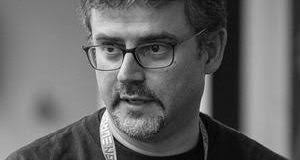
\includegraphics[width=.5\textwidth]{pics/alberto_brandolini.jpg} };
\end{tikzpicture}

\onslide+<2->
 \begin{tikzpicture}
            \put (100,-80) { 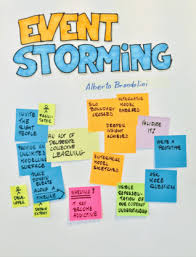
\includegraphics[height=.5\textheight]{pics/eventstorming.jpg} };
\end{tikzpicture}

\onslide+<3->
 \begin{tikzpicture}
            \put (180,-120) { 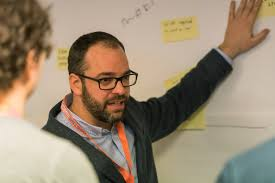
\includegraphics[width=.5\textwidth]{pics/mathias_verraes.jpg} };
\end{tikzpicture}

\end{frame}

%%%%%%%%%%%%%%%%%%%%%%%%%%%%%%%%%%%%%%%%%%%%%%%%%%%
%\begin{frame}[fragile]{}
%
%\begin{itemize}
%\item Wenig Domain-Driven Design
%\item Viel gemeinsames Verständnis
%\begin{itemize}
%\item Knowledge Crunching
%\item mit EventStorming
%\end{itemize}
%\end{itemize}
%
%\end{frame}

\numberednote{
Standing on the shoulders of giants

~\\

Das möchte ich Euch heute vorstellen

\begin{itemize}
\item Wenig Domain-Driven Design
\item Viel gemeinsames Verständnis
\begin{itemize}
\item Knowledge Crunching
\item mit EventStorming
\end{itemize}
\end{itemize}

EventStorming: sehr schnell sehr detailliertes Modell
}


%%%%%%%%%%%%%%%%%%%%%%%%%%%%%%%%%%%%%%%%%%%%%%%%%%
\begin{frame}[fragile]{Gemeinsames Verständnis schaffen - Warum?}

\begin{itemize}
\item Gedanken sichtbar und ``begreifbar'' machen
\item Modell schafft Klarheit
\item Ubiquitous Language grenzt Begriffe ab
\end{itemize}

\end{frame}

\numberednote{

Jeder entwickelt eigene Vorstellung von etwas Gehörtem

}

%%%%%%%%%%%%%%%%%%%%%%%%%%%%%%%%%%%%%%%%%%%%%%%%%%
\begin{frame}[fragile]{}

 \begin{tikzpicture}[remember picture,overlay]
            \node[at=(current page.center)] {
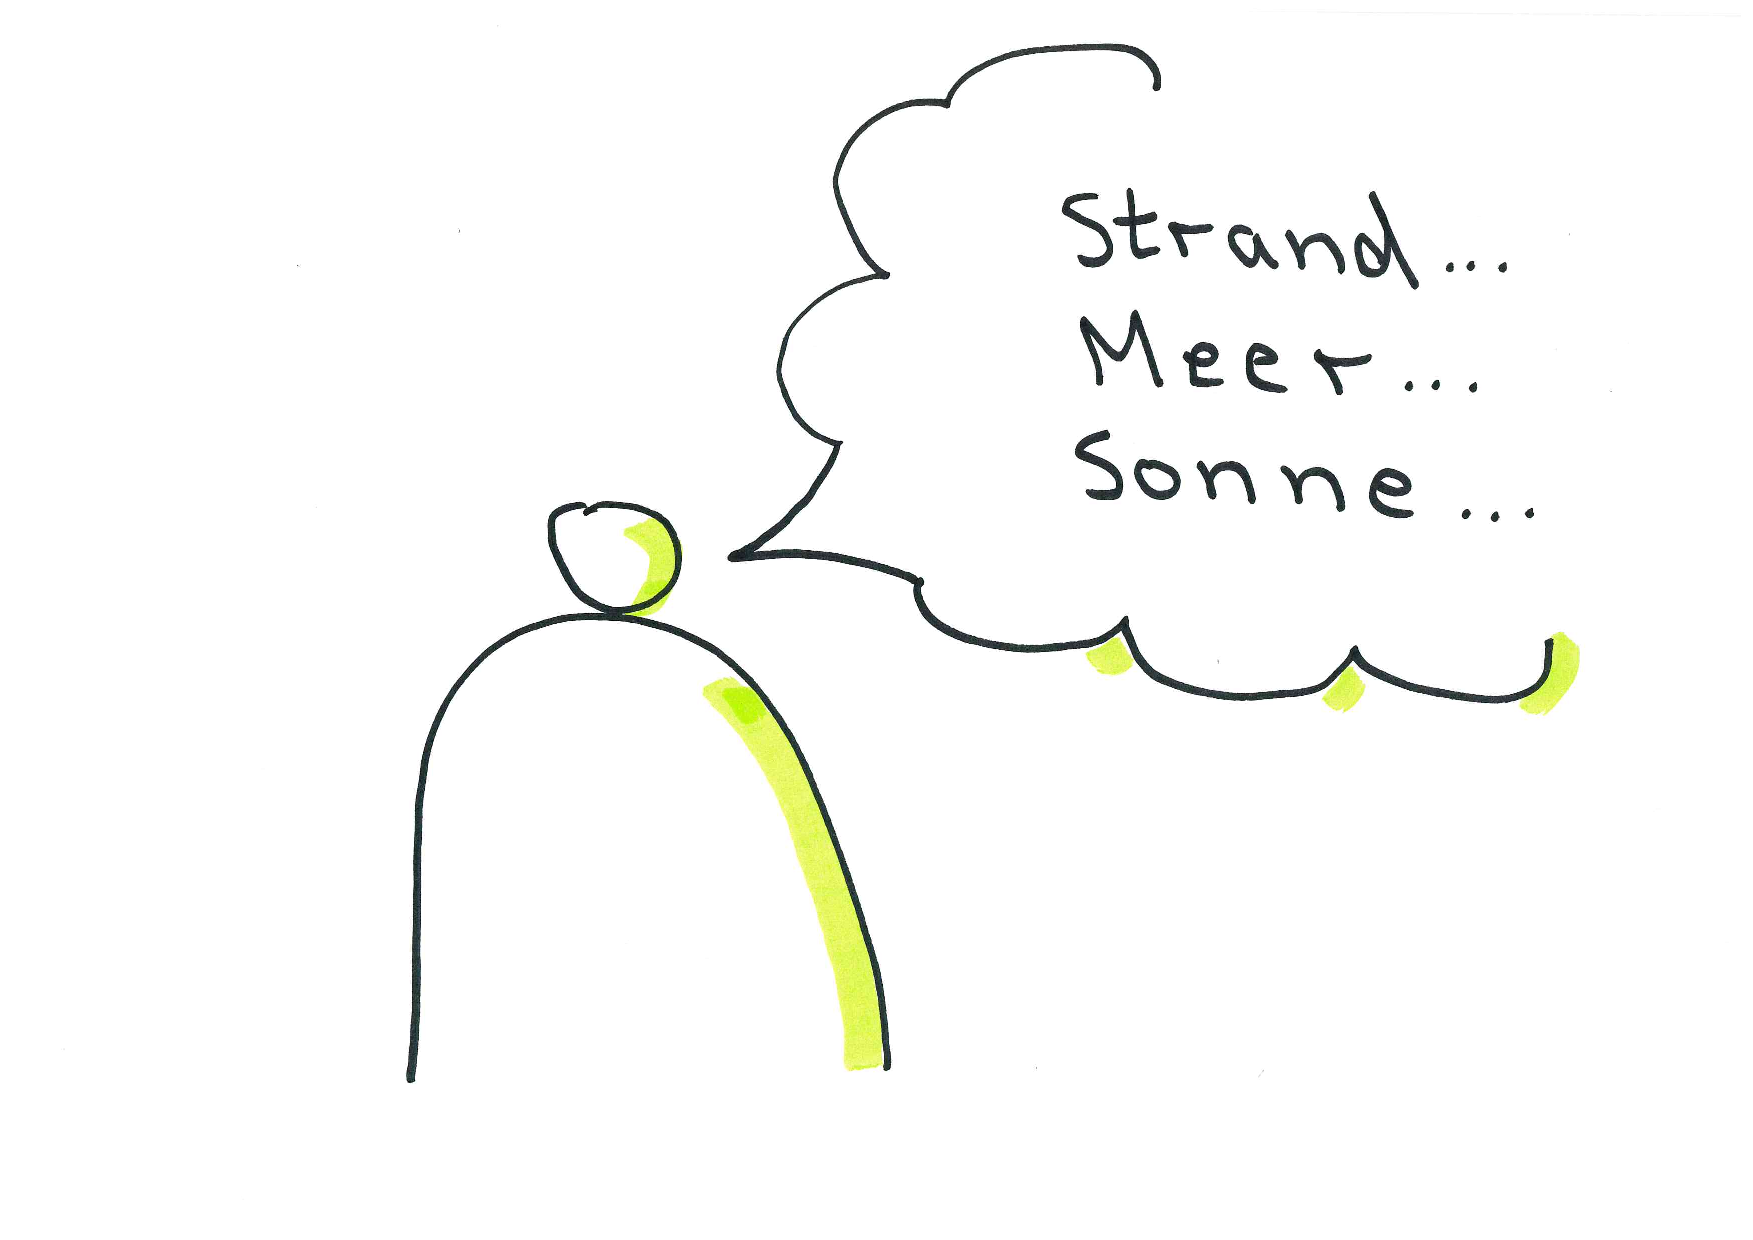
\includegraphics[height=\paperheight]{pics/ich_berichte_von_meinem_urlaub.jpg} % sonne, strand, meer
            };
\end{tikzpicture}

\end{frame}

\numberednote{

\begin{itemize}
\item sonne stand am himmel, strand breitete sich vor mir aus, meer schwappte sanft ans ufer
\item jeder von euch hat wahrscheinlich ein bild im kopf
\item vielleicht sieht euer bild so oder so ähnlich aus
\item vielleicht war ich aber gar nicht allein, sondern in Gesellschaft
\item vielleicht war ich auch in einem anderen kulturkreis
\item oder vielleicht in einer anderen Klimazone
\end{itemize}

auf alle diese bilder passt die beschreibung von sonne, strand und meer

}


%%%%%%%%%%%%%%%%%%%%%%%%%%%%%%%%%%%%%%%%%%%%%%%%%%
\begin{frame}[fragile]{}

 \begin{tikzpicture}[remember picture,overlay]
            \node[at=(current page.center)] {
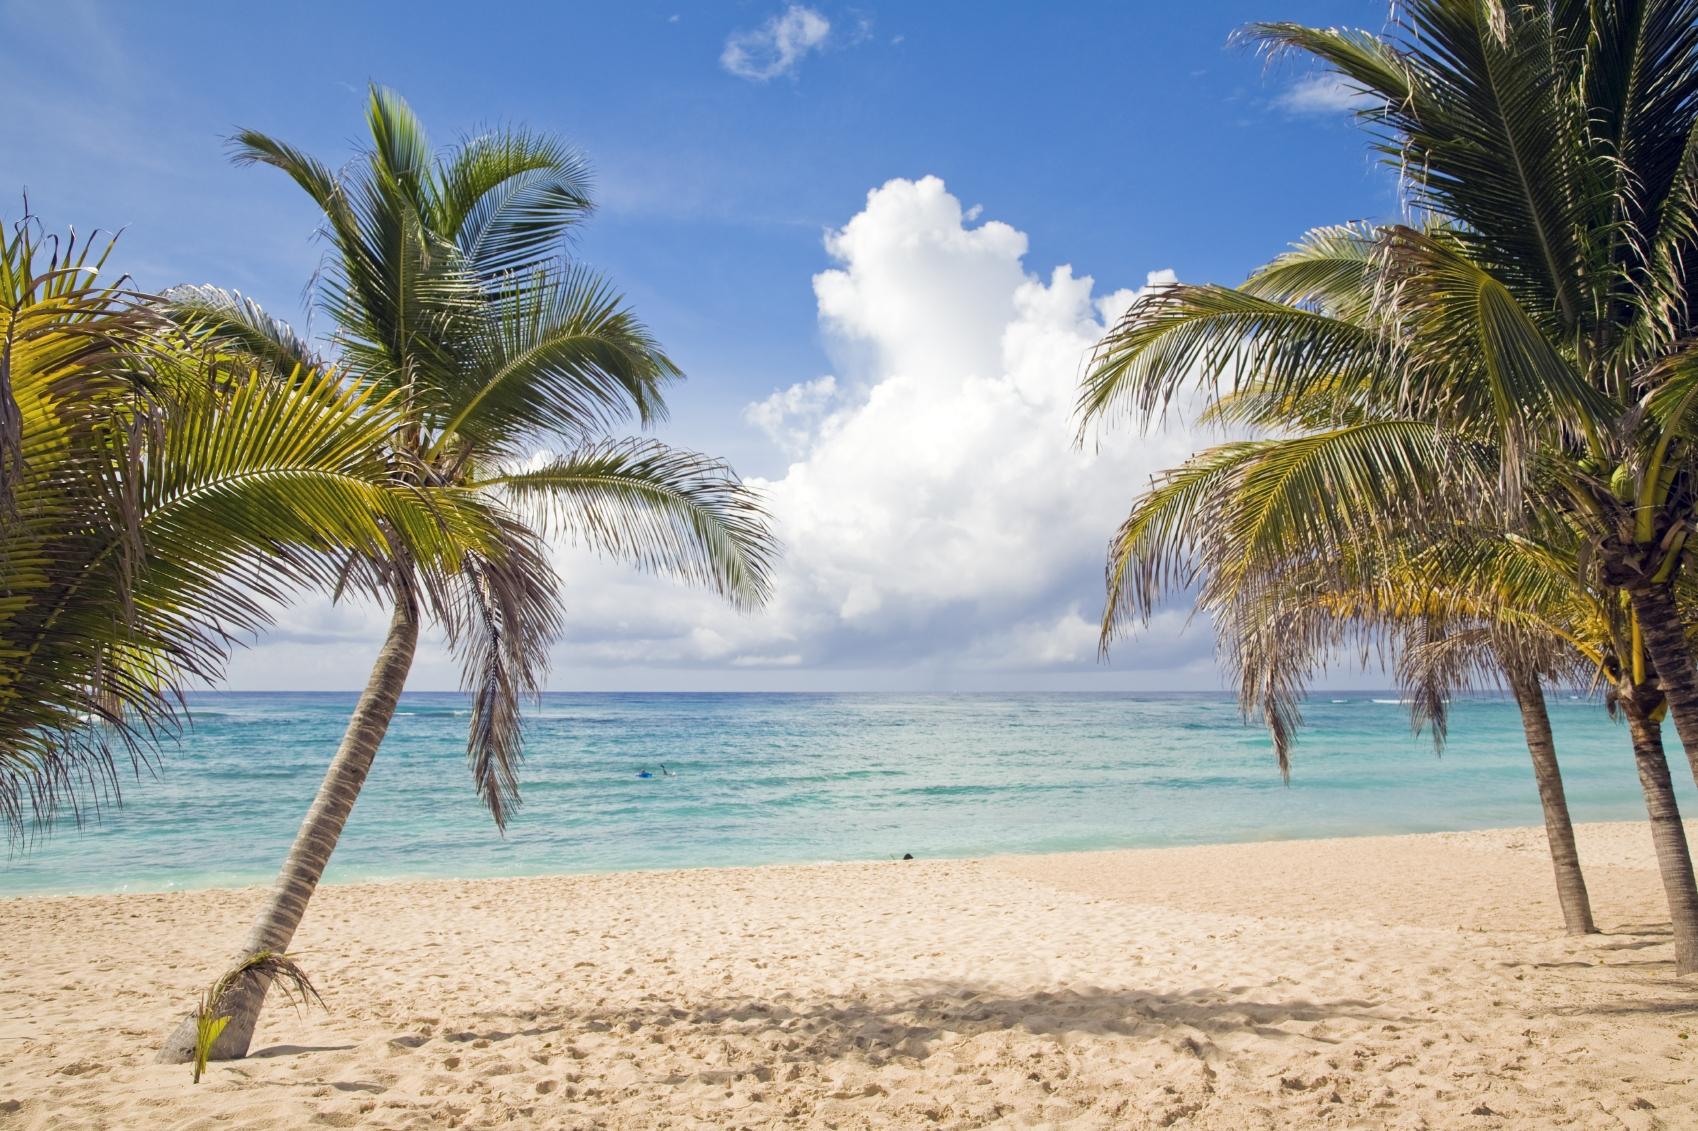
\includegraphics[height=\paperheight]{pics/palm_beach.jpg}
            };
\end{tikzpicture}

\end{frame}

%%%%%%%%%%%%%%%%%%%%%%%%%%%%%%%%%%%%%%%%%%%%%%%%%%
\begin{frame}[fragile]{}

 \begin{tikzpicture}[remember picture,overlay]
            \node[at=(current page.center)] {
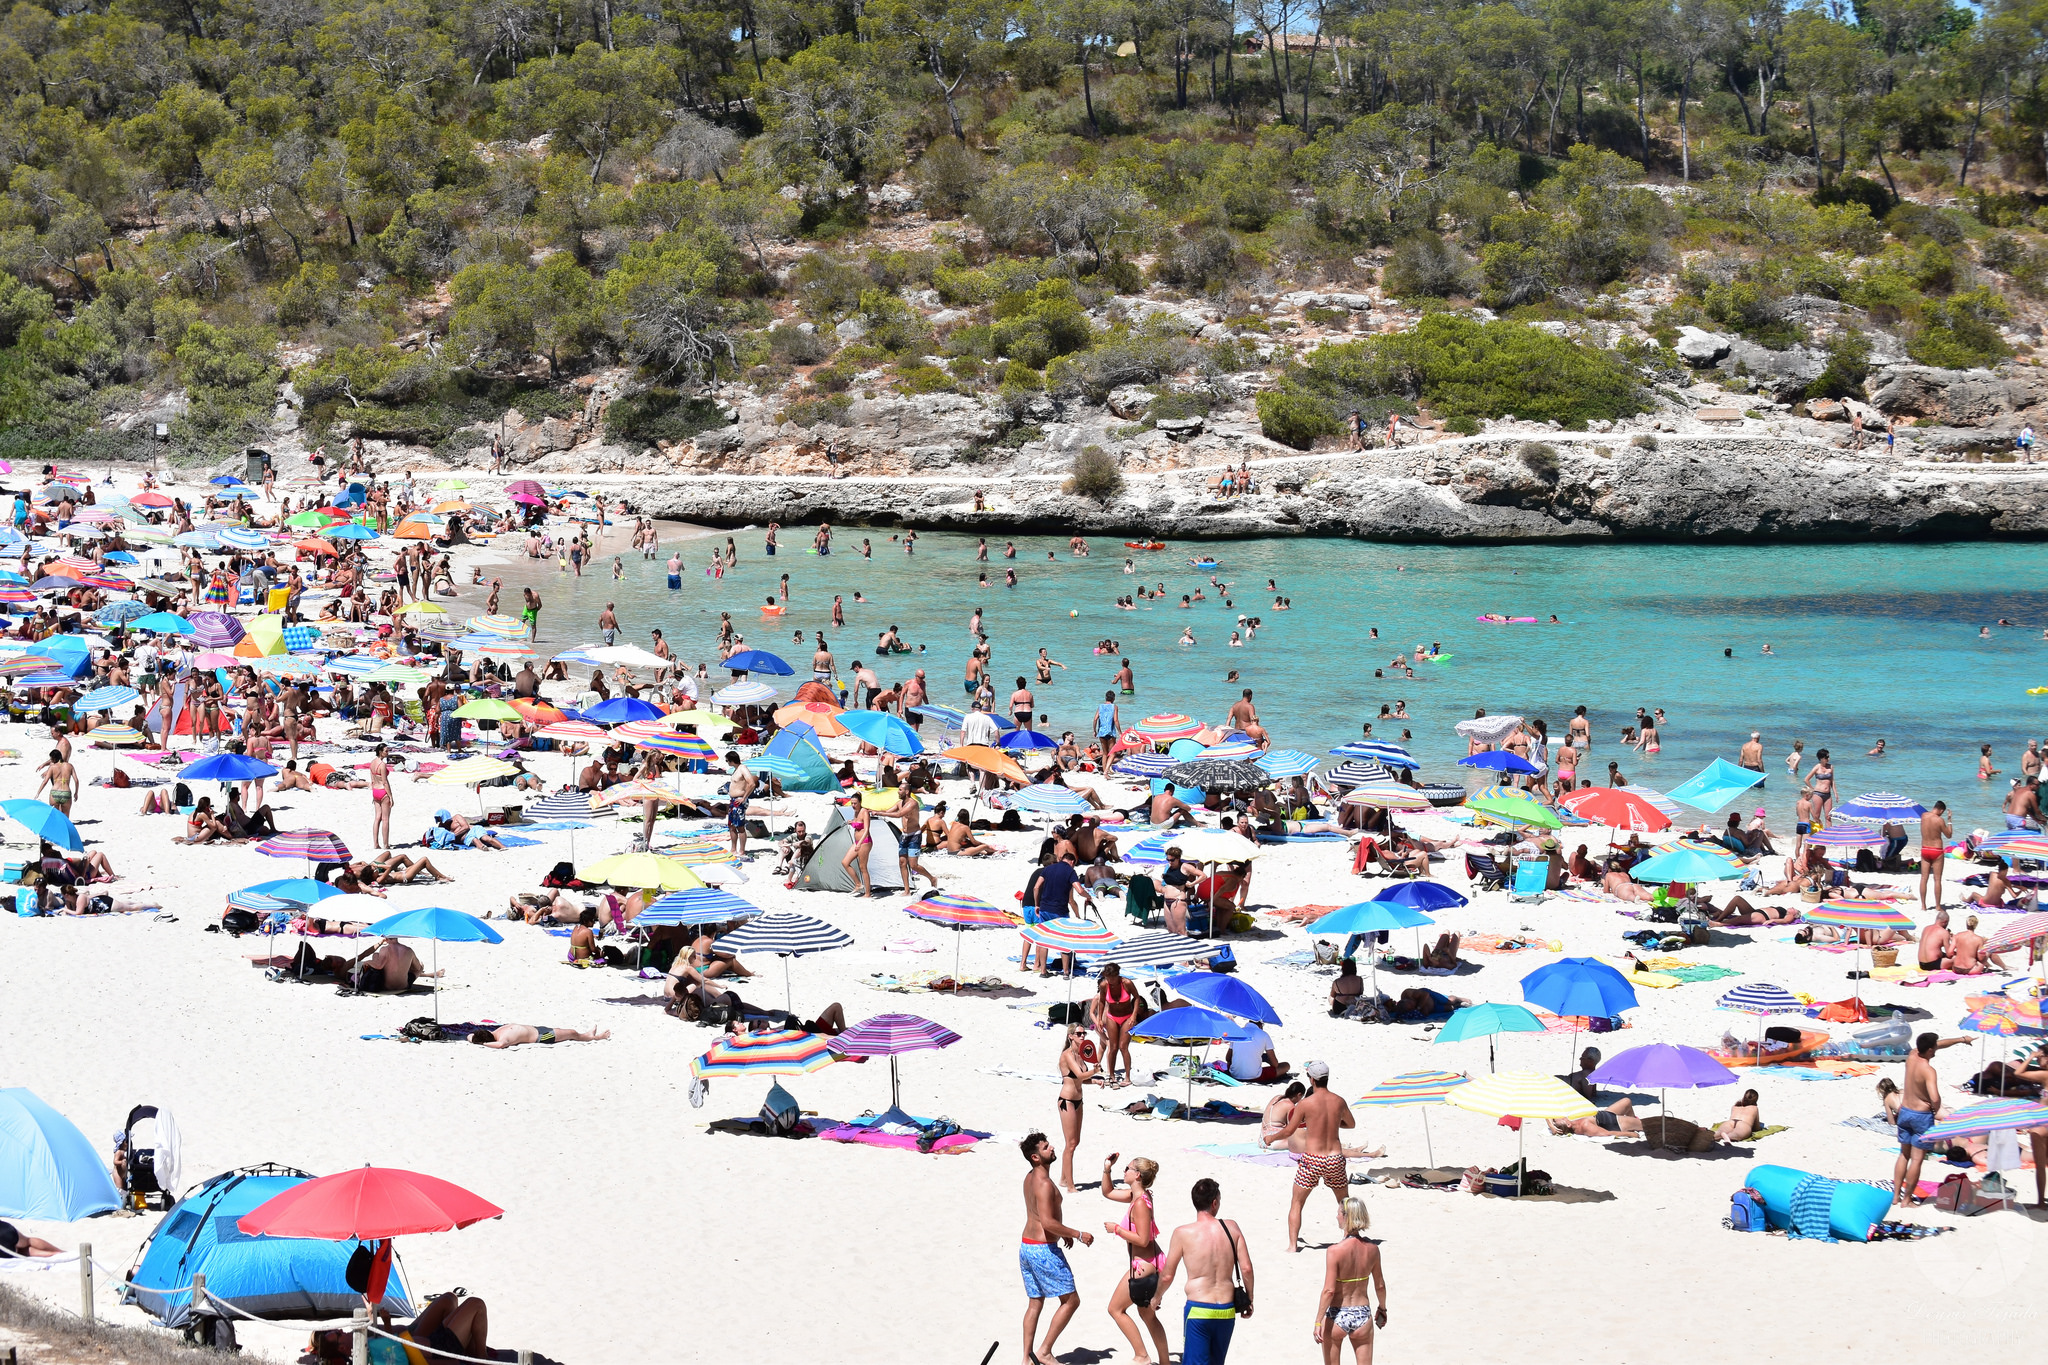
\includegraphics[height=\paperheight]{pics/mallorca_beach.jpg}
            };
\end{tikzpicture}

\end{frame}

%%%%%%%%%%%%%%%%%%%%%%%%%%%%%%%%%%%%%%%%%%%%%%%%%%
\begin{frame}[fragile]{}

 \begin{tikzpicture}[remember picture,overlay]
            \node[at=(current page.center)] {
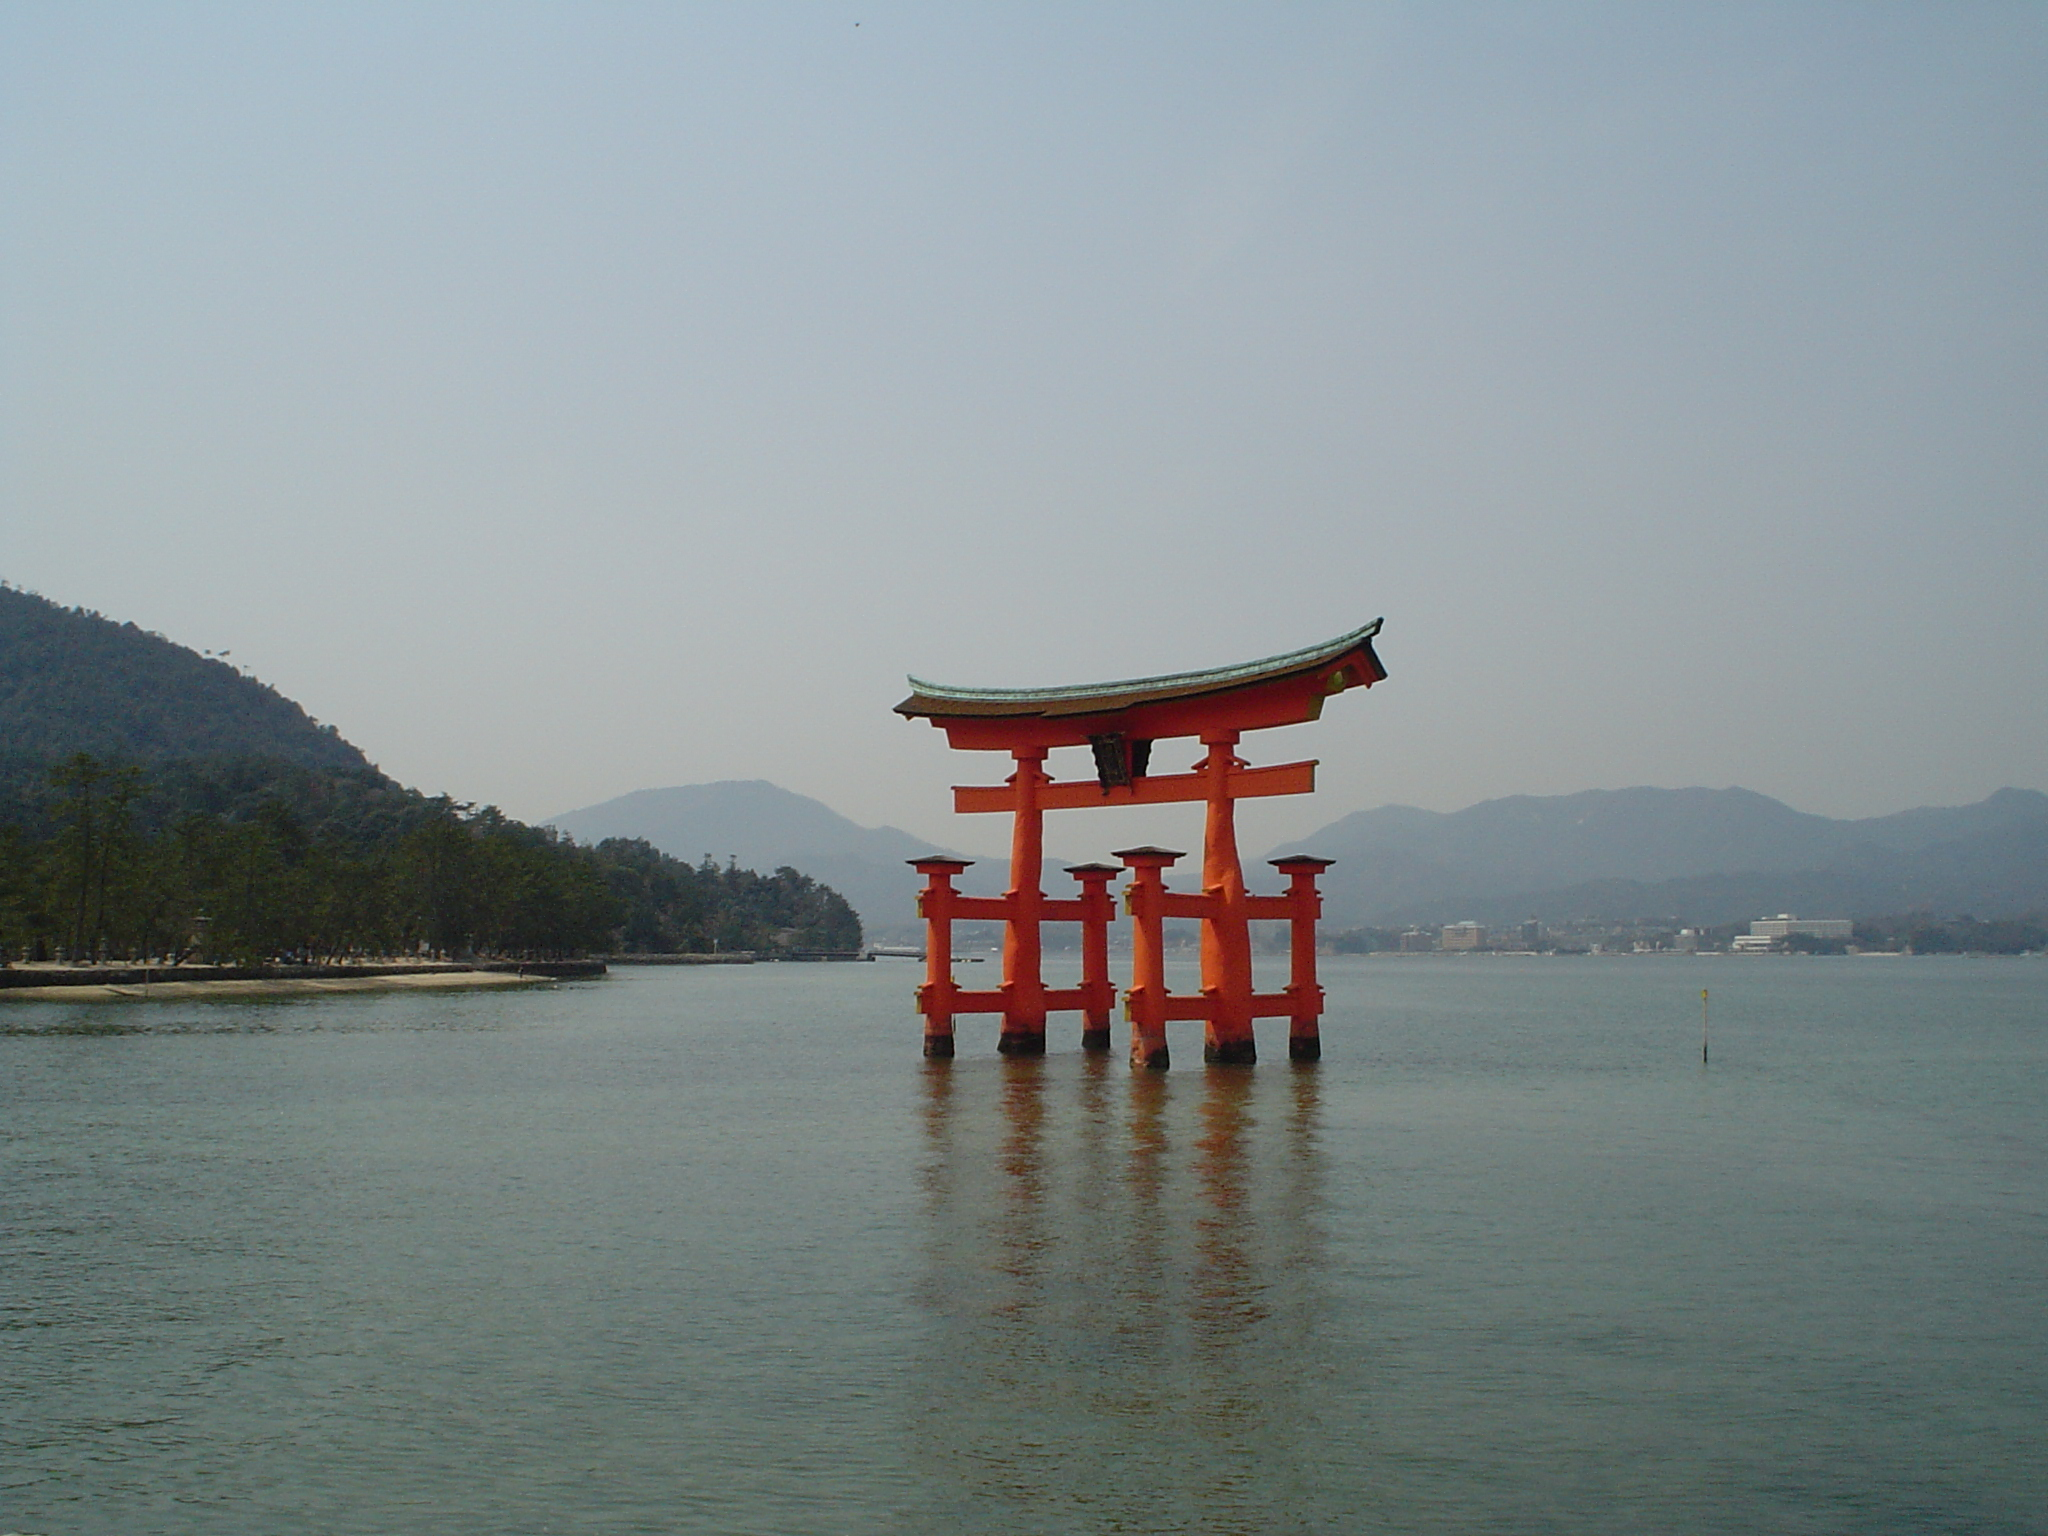
\includegraphics[height=\paperheight]{pics/japan_beach.jpg}
            };
\end{tikzpicture}

\end{frame}

%%%%%%%%%%%%%%%%%%%%%%%%%%%%%%%%%%%%%%%%%%%%%%%%%%
\begin{frame}[fragile]{}

 \begin{tikzpicture}[remember picture,overlay]
            \node[at=(current page.center)] {
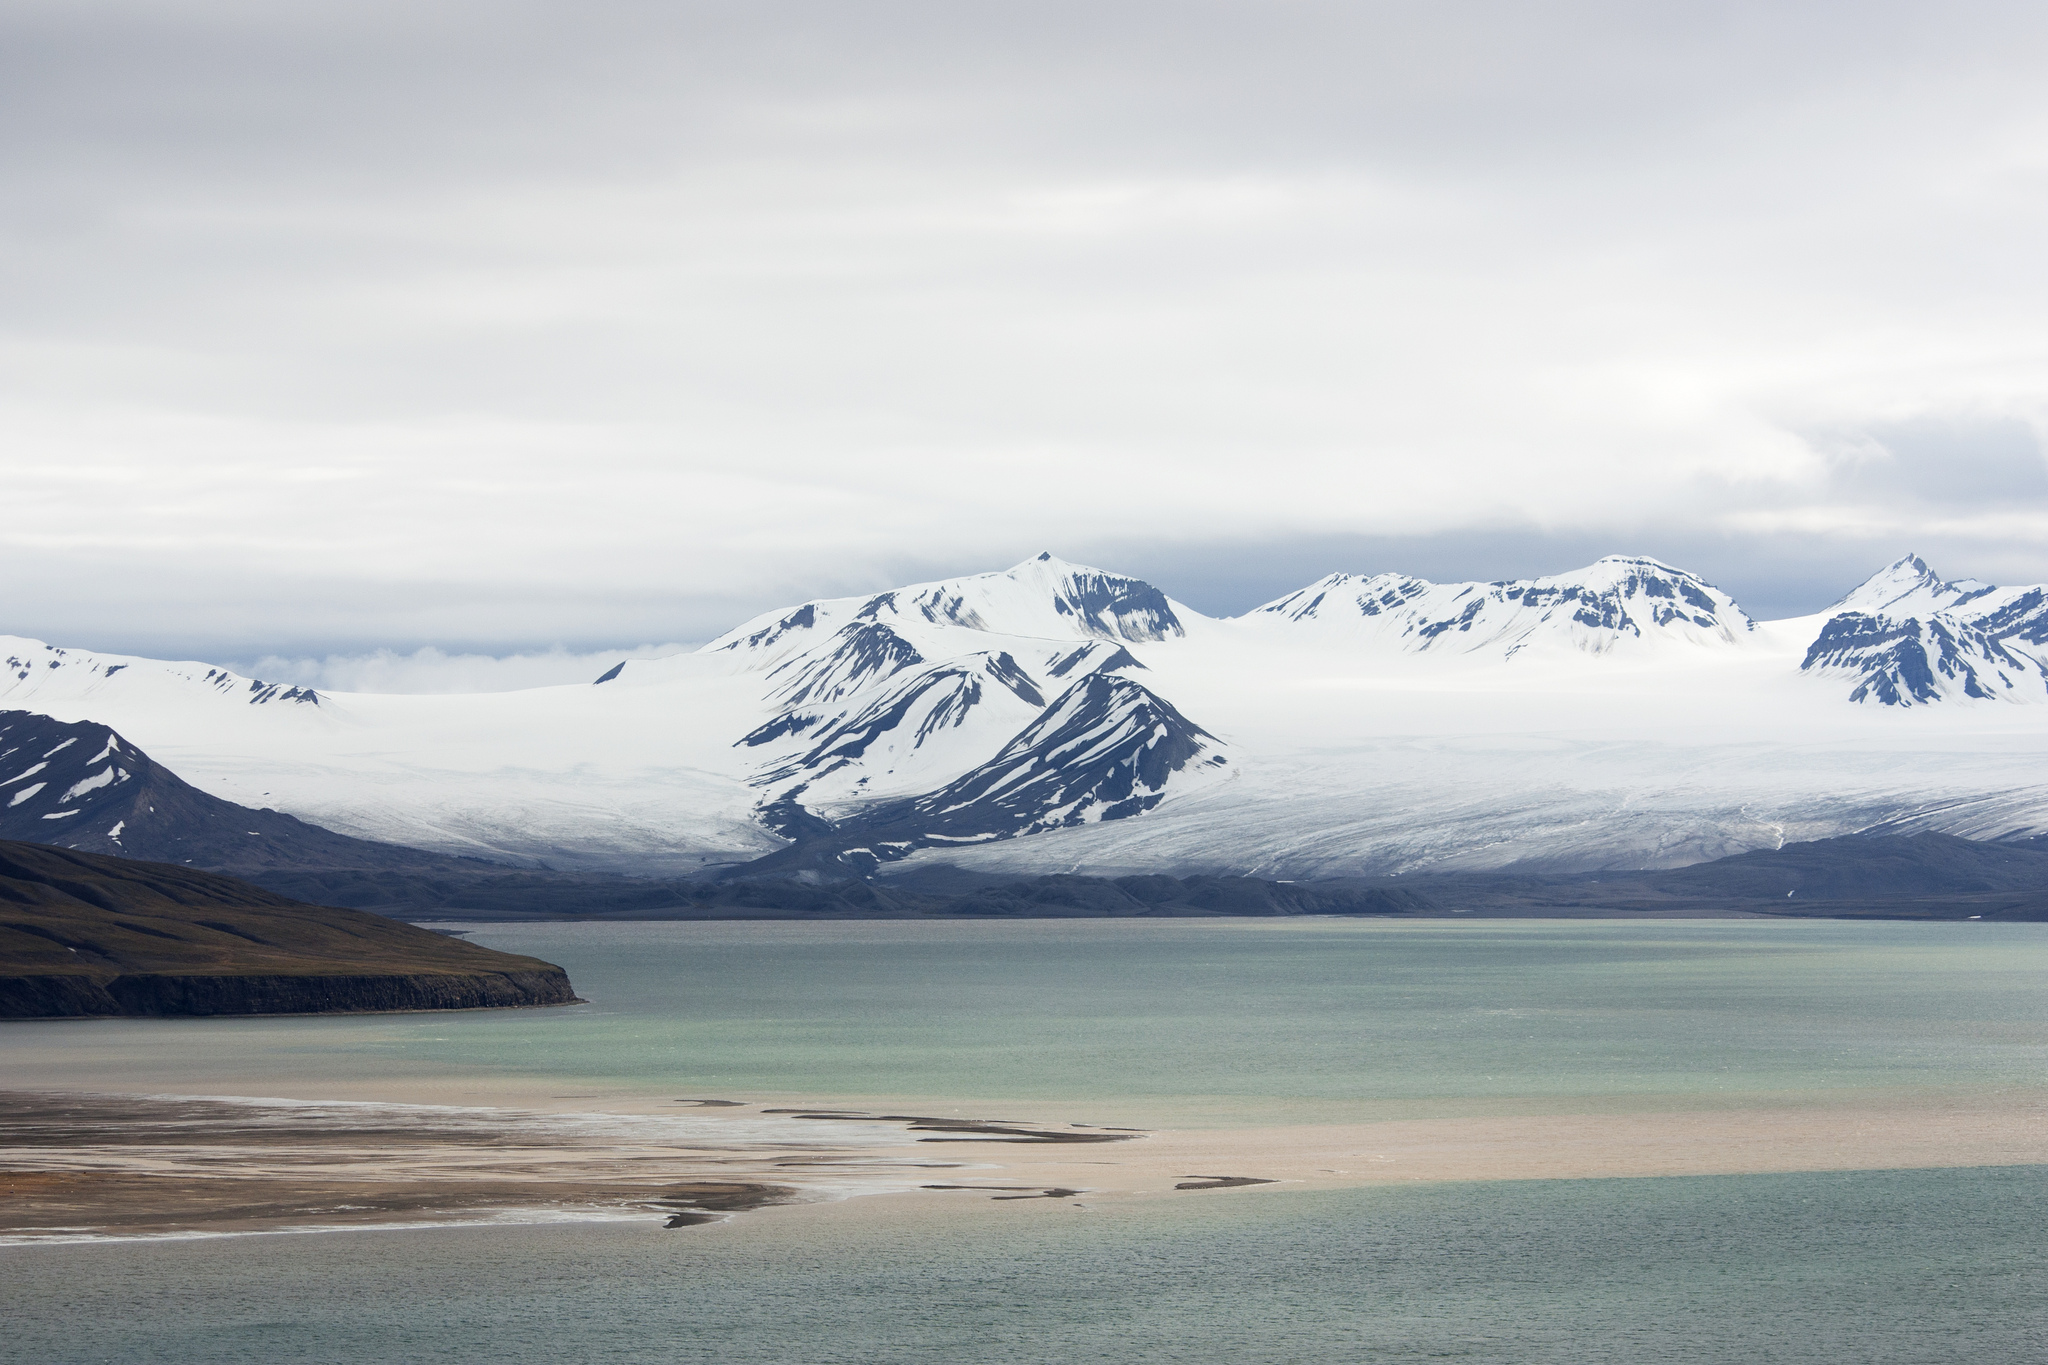
\includegraphics[height=\paperheight]{pics/ice_beach.jpg}
            };
\end{tikzpicture}

\end{frame}

%%%%%%%%%%%%%%%%%%%%%%%%%%%%%%%%%%%%%%%%%%%%%%%%%%
\begin{frame}[fragile]{}

 \begin{tikzpicture}[remember picture,overlay]
            \node[at=(current page.center)] {
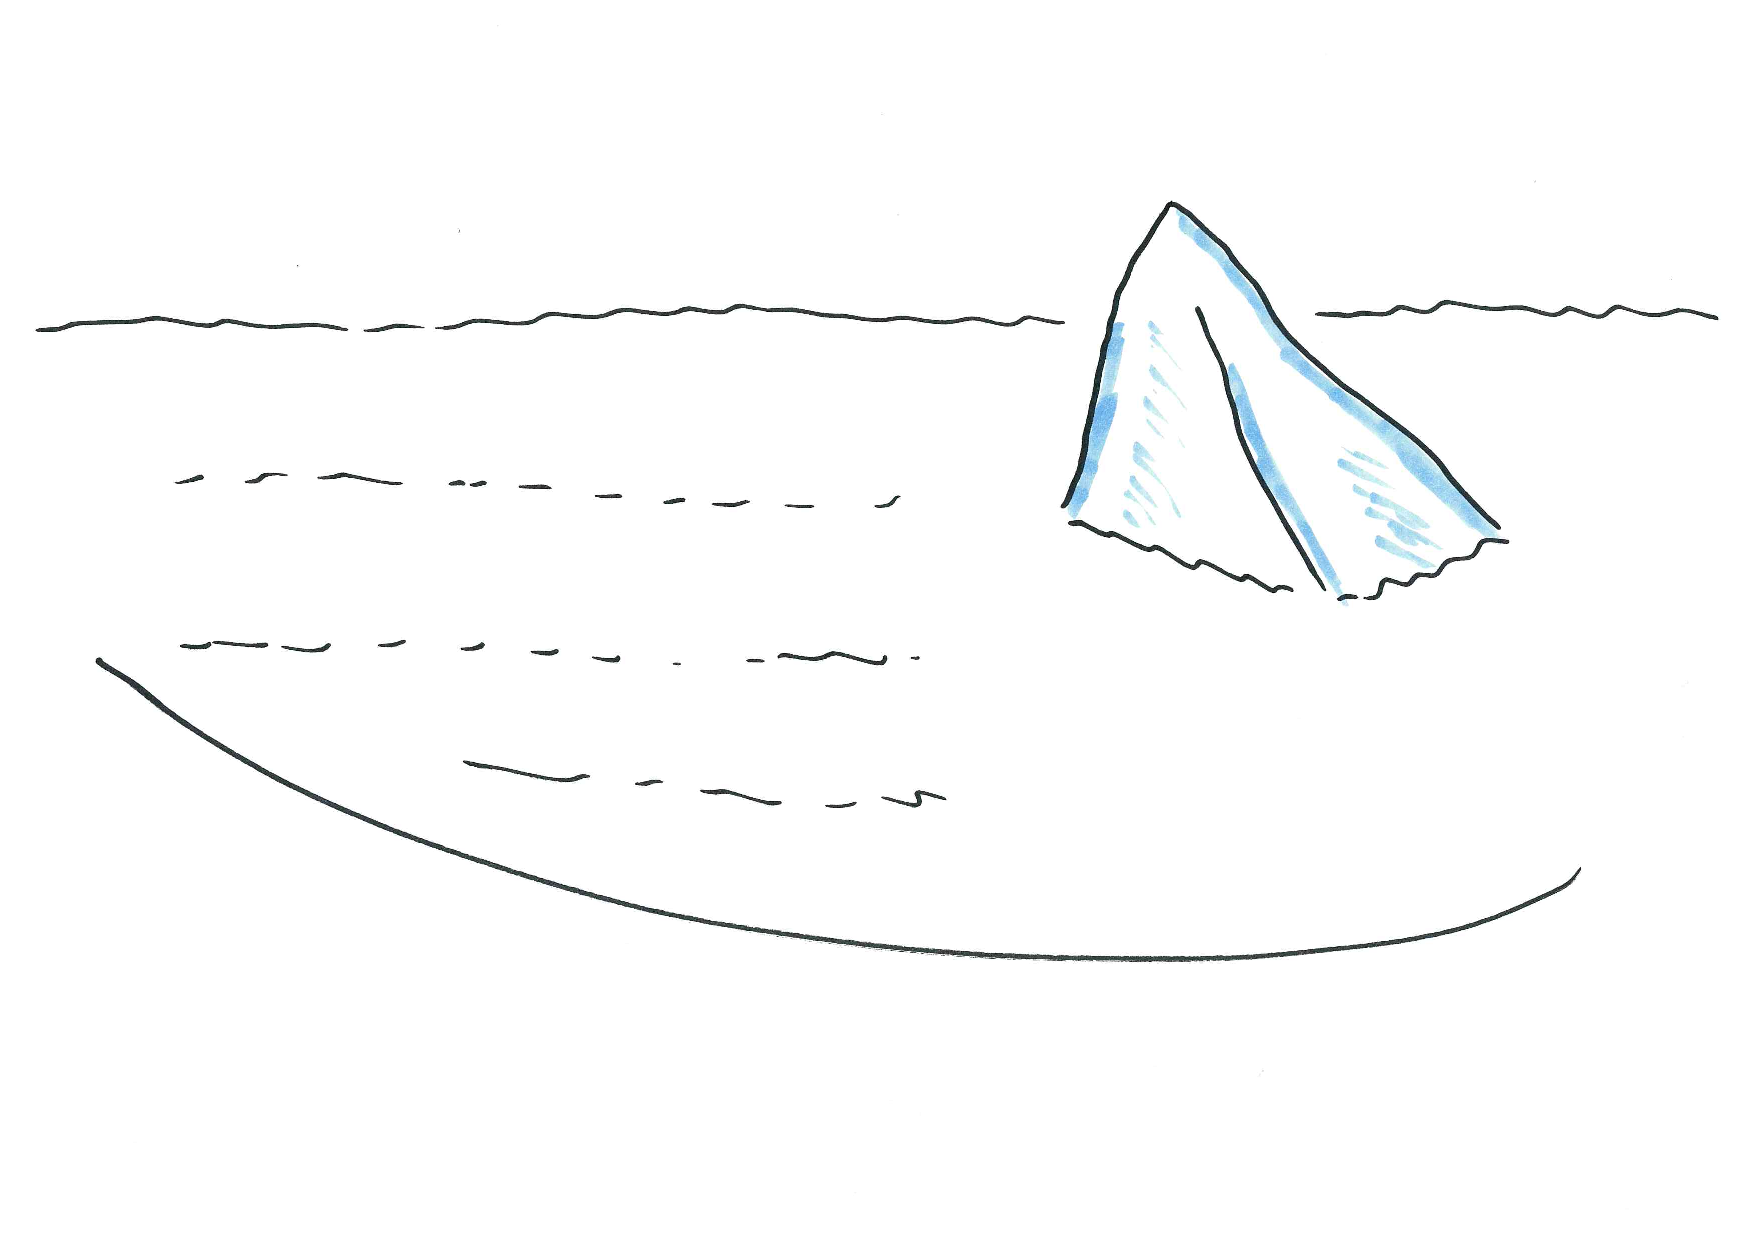
\includegraphics[height=\paperheight]{pics/eine_skizze_meines_urlaubs.jpg}
            };
\end{tikzpicture}

\end{frame}

\numberednote{

\begin{itemize}
\item wenn ich eine skizze meines urlaubs male, dann gibt es euch vielleicht eine chance, Rückfragen zu stellen und dinge zu klären

\item was ist das da für ein felsen im wasser, und wieso ist der blau? -> Das ist kein Felsen, sondern ein Eisberg.

\item Offensichtliches bleibt gern unerwähnt.
\end{itemize}
}

%%%%%%%%%%%%%%%%%%%%%%%%%%%%%%%%%%%%%%%%%%%%%%%%%%
\begin{frame}[fragile]{WARNUNG}

\begin{center}
{
\LARGE
Hier bei uns passiert gerade dasselbe!
}
\end{center}

\end{frame}

\numberednote{
Vieles, was ich sage, versteht Ihr vermutlich anders als ich es erwarte
}

%%%%%%%%%%%%%%%%%%%%%%%%%%%%%%%%%%%%%%%%%%%%%%%%%%
\begin{frame}[fragile]{}

\begin{center}
{
\LARGE
WORKSHOP}
\end{center}

\end{frame}


%%%%%%%%%%%%%%%%%%%%%%%%%%%%%%%%%%%%%%%%%%%%%%%%%%
\begin{frame}[fragile]{Unsere Domäne: eCommerce}

\onslide+<2->
 \begin{tikzpicture}
 % x (kleiner = weiter nach links) y (kleiner = weiter nach unten)
            \put (-10,-20) { 
\includegraphics[width=.4\textwidth]{pics/onlineshopping.png} };
\end{tikzpicture}

\onslide+<3->
 \begin{tikzpicture}
            \put (90,-120) { 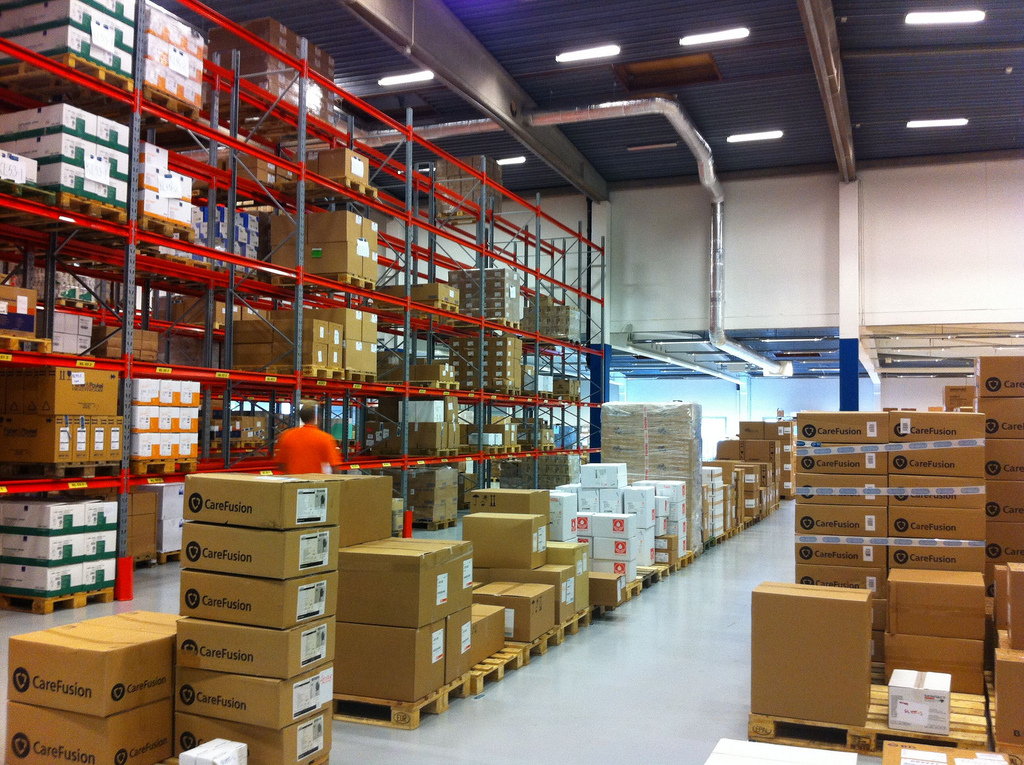
\includegraphics[height=.4\textheight]{pics/warehouse.jpg} };
\end{tikzpicture}

\onslide+<4->
 \begin{tikzpicture}
            \put (180,30) { 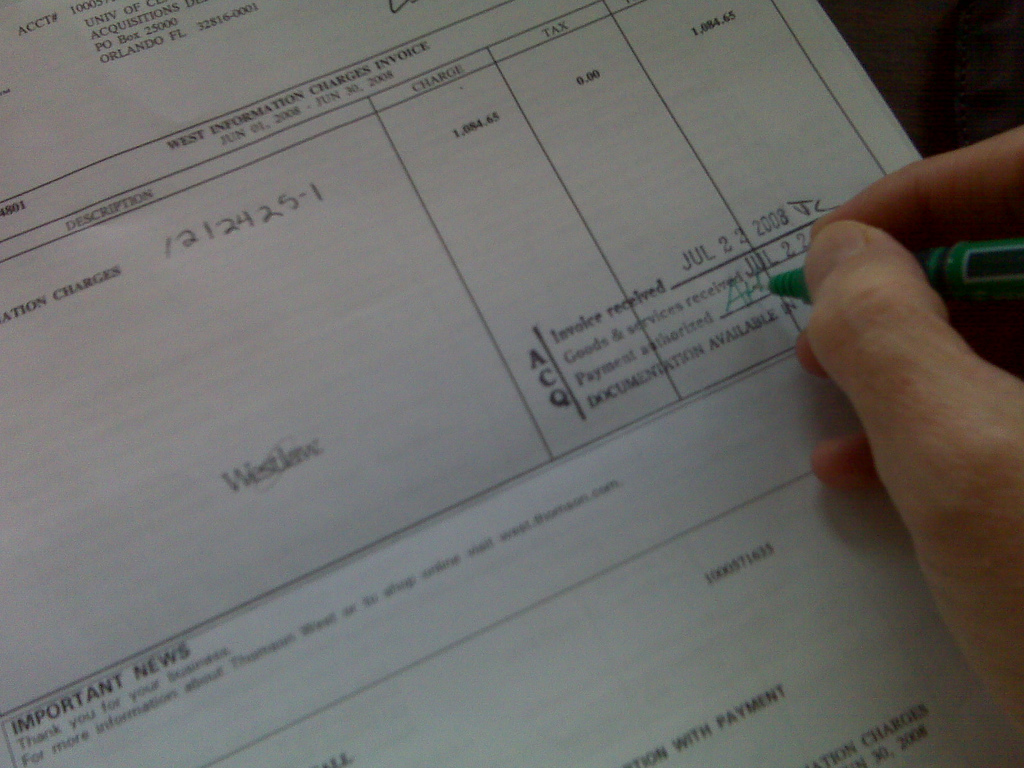
\includegraphics[width=.4\textwidth]{pics/ordering.jpg} };
\end{tikzpicture}

\end{frame}

\numberednote{
\begin{itemize}
\item Onlineshop
\item Lagerhaltung
\item Bestellungen
\end{itemize}
}

%%%%%%%%%%%%%%%%%%%%%%%%%%%%%%%%%%%%%%%%%%%%%%%%%%
%%%%%%%%%%%%%%%%%%%%%%%%%%%%%%%%%%%%%%%%%%%%%%%%%%
\begin{frame}[fragile]{EventStorming I}

\textbf{Events} erfassen

\begin{itemize}
\item Ereignis in der Vergangenheit
\item Relevant für den Fachbereich
\item Beobachtbar im System
\end{itemize}

\onslide+<2->
\begin{itemize}
\item Beschrieben durch \textbf{Verb in der Vergangenheit}
\end{itemize}

\end{frame}

%%%%%%%%%%%%%%%%%%%%%%%%%%%%%%%%%%%%%%%%%%%%%%%%%%
\begin{frame}[fragile]{Beispiel}

\begin{center}

\includegraphics[width=.5\textwidth]{pics/eventstorming1.jpg}
\end{center}

\end{frame}


%%%%%%%%%%%%%%%%%%%%%%%%%%%%%%%%%%%%%%%%%%%%%%%%%%%
%\begin{frame}[fragile]{Übung}
%
%Erfassen Sie die Events der Domäne \glqq eCommerce\grqq !
%
%\end{frame}


%%%%%%%%%%%%%%%%%%%%%%%%%%%%%%%%%%%%%%%%%%%%%%%%%%
%\begin{frame}[fragile]{Was kann schiefgehen?}
\numberednote{

\textbf{Übung:} Events der Domäne erfassen! (20 - 30 min)

~\\
\textbf{Was kann schiefgehen:}

\begin{itemize}
\item kein Verb
\item nicht in der Vergangenheit
\item außerhalb des Beobachtbaren
\begin{itemize}
\item Kunde beginnt sich für unsere Produkte zu interessieren
\item Kunde erhält seine Lieferung
\end{itemize}
\end{itemize}

}
%\end{frame}


%%%%%%%%%%%%%%%%%%%%%%%%%%%%%%%%%%%%%%%%%%%%%%%%%%
%%%%%%%%%%%%%%%%%%%%%%%%%%%%%%%%%%%%%%%%%%%%%%%%%%
\begin{frame}[fragile]{EventStorming II}

\begin{itemize}
\item Viele Events unterliegen einer zeitlichen Abfolge
\item Zeit verläuft \textbf{von links nach rechts}
\end{itemize}

\end{frame}

%%%%%%%%%%%%%%%%%%%%%%%%%%%%%%%%%%%%%%%%%%%%%%%%%%
\begin{frame}[fragile]{Zeit}

\begin{center}
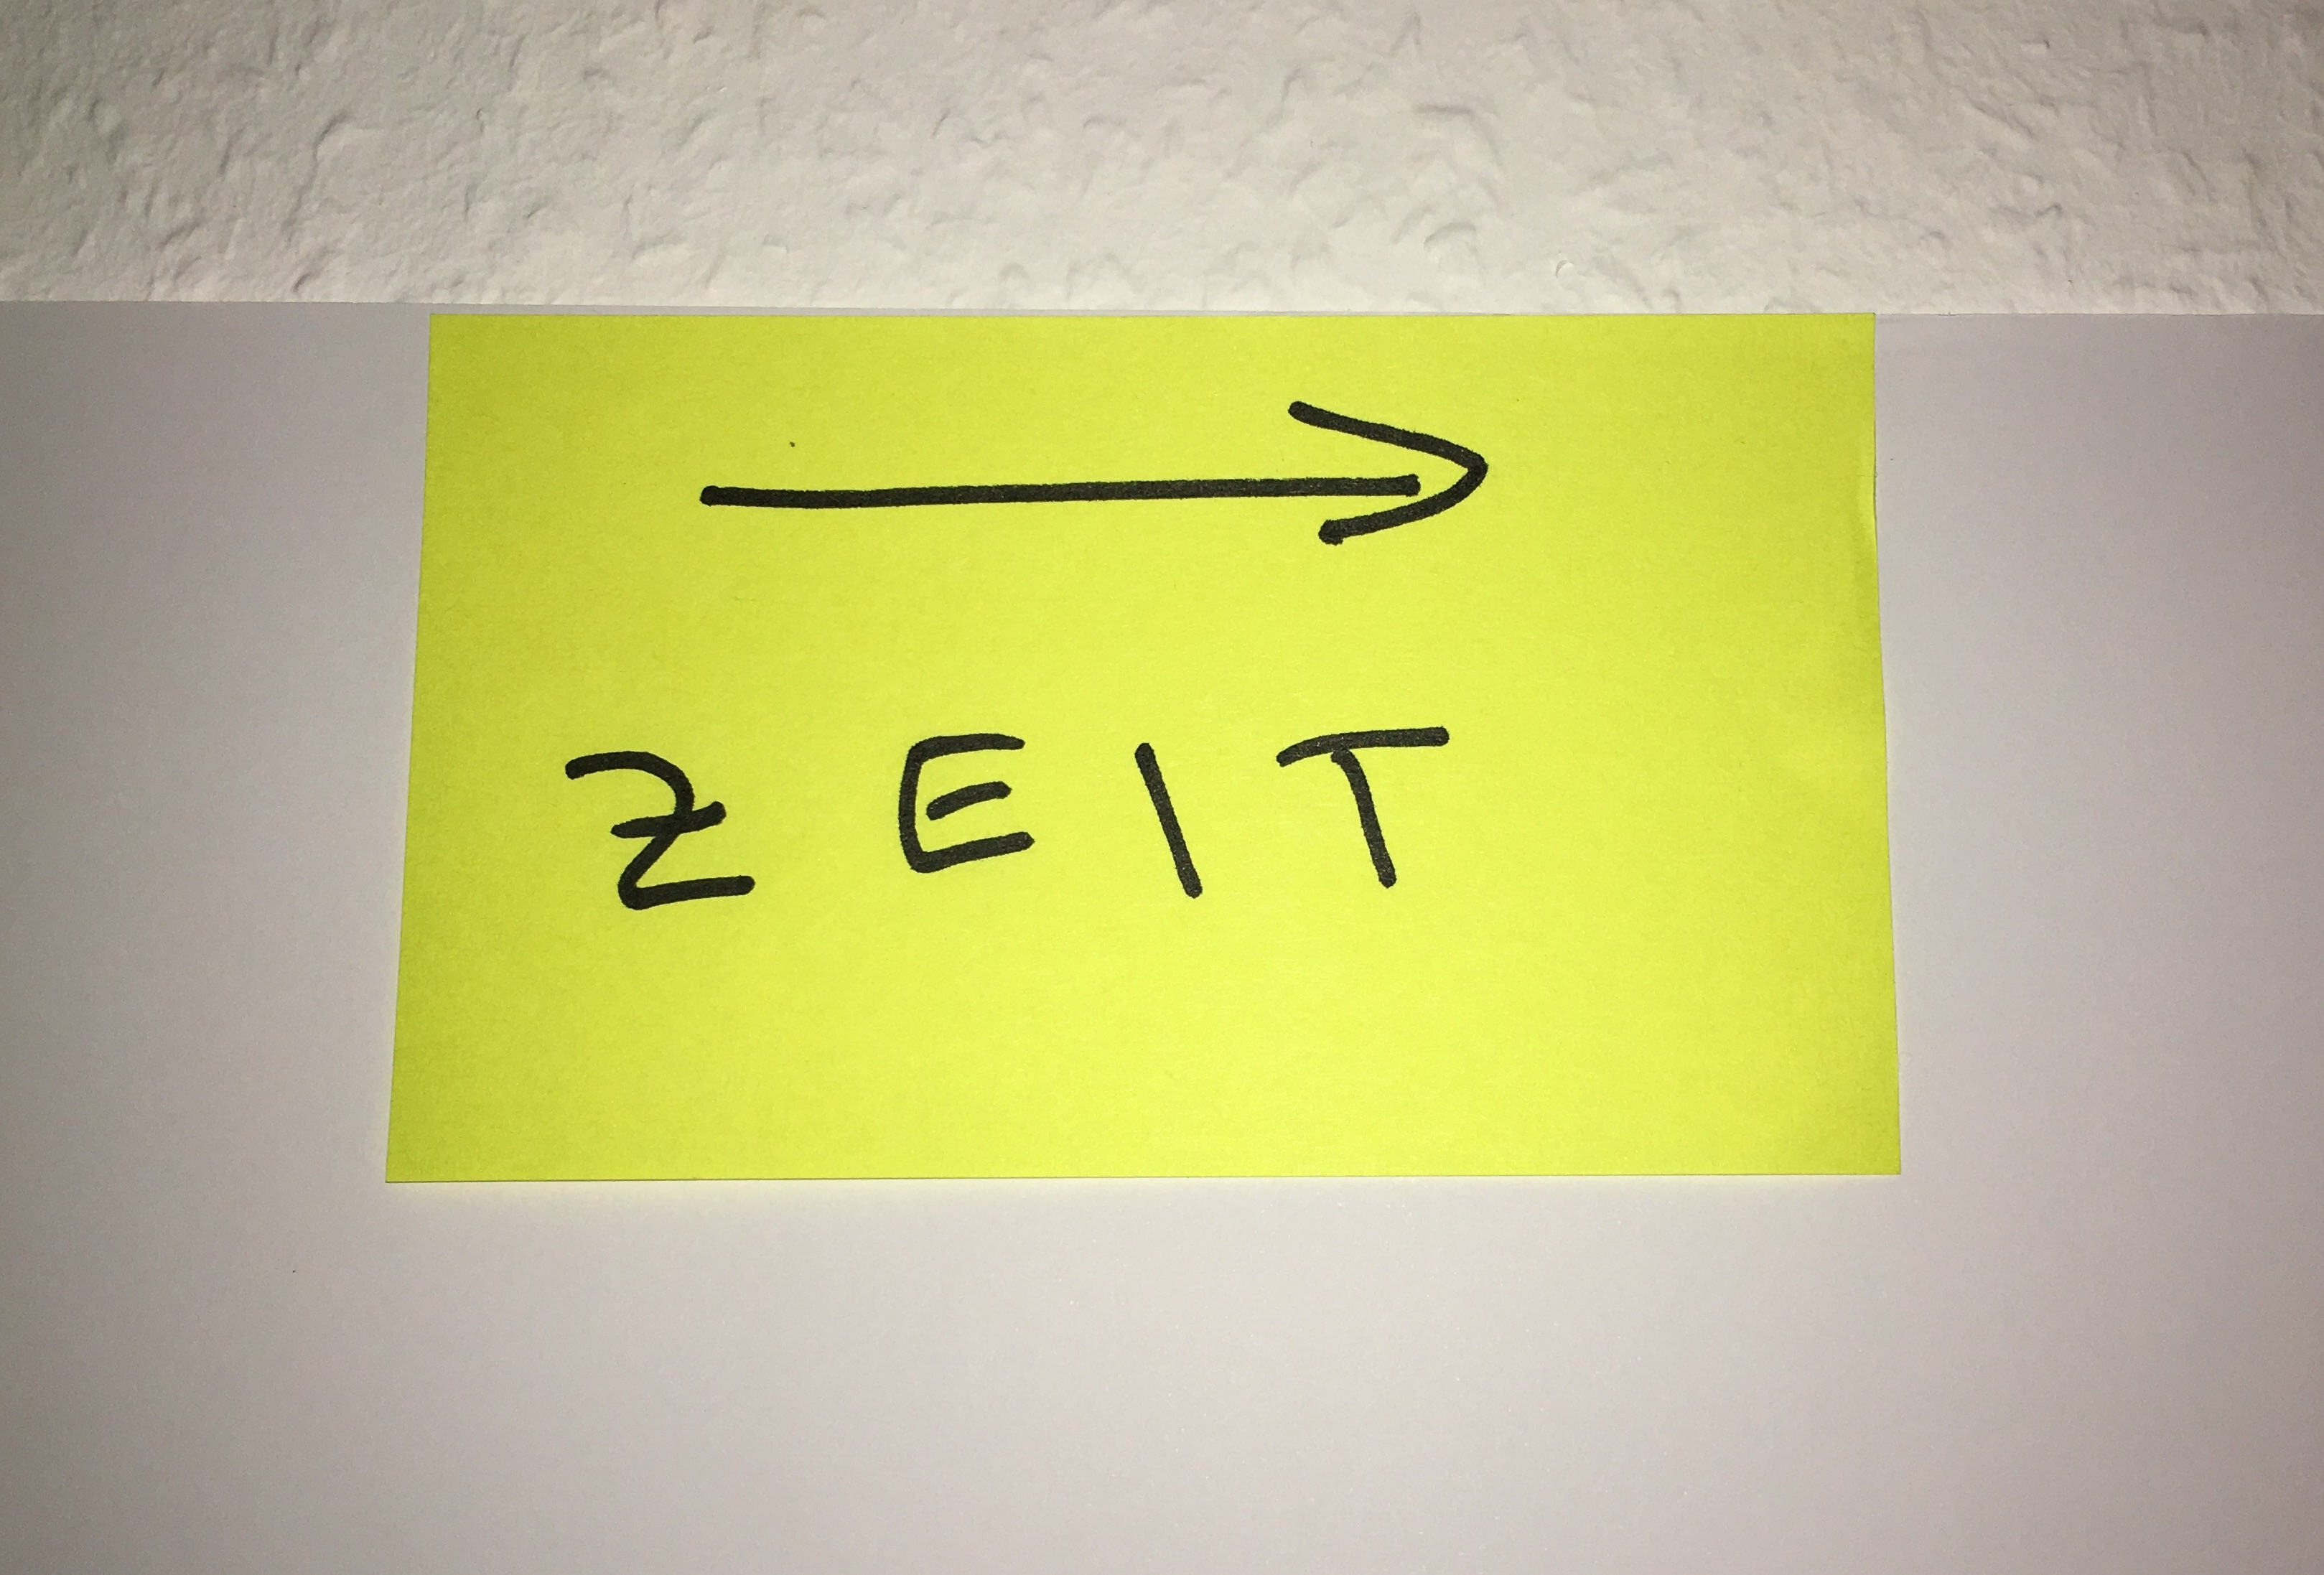
\includegraphics[width=.5\textwidth]{pics/eventstorming_zeit.jpg}
\end{center}

\end{frame}


%%%%%%%%%%%%%%%%%%%%%%%%%%%%%%%%%%%%%%%%%%%%%%%%%%
\begin{frame}[fragile]{Beispiel}

\begin{center}
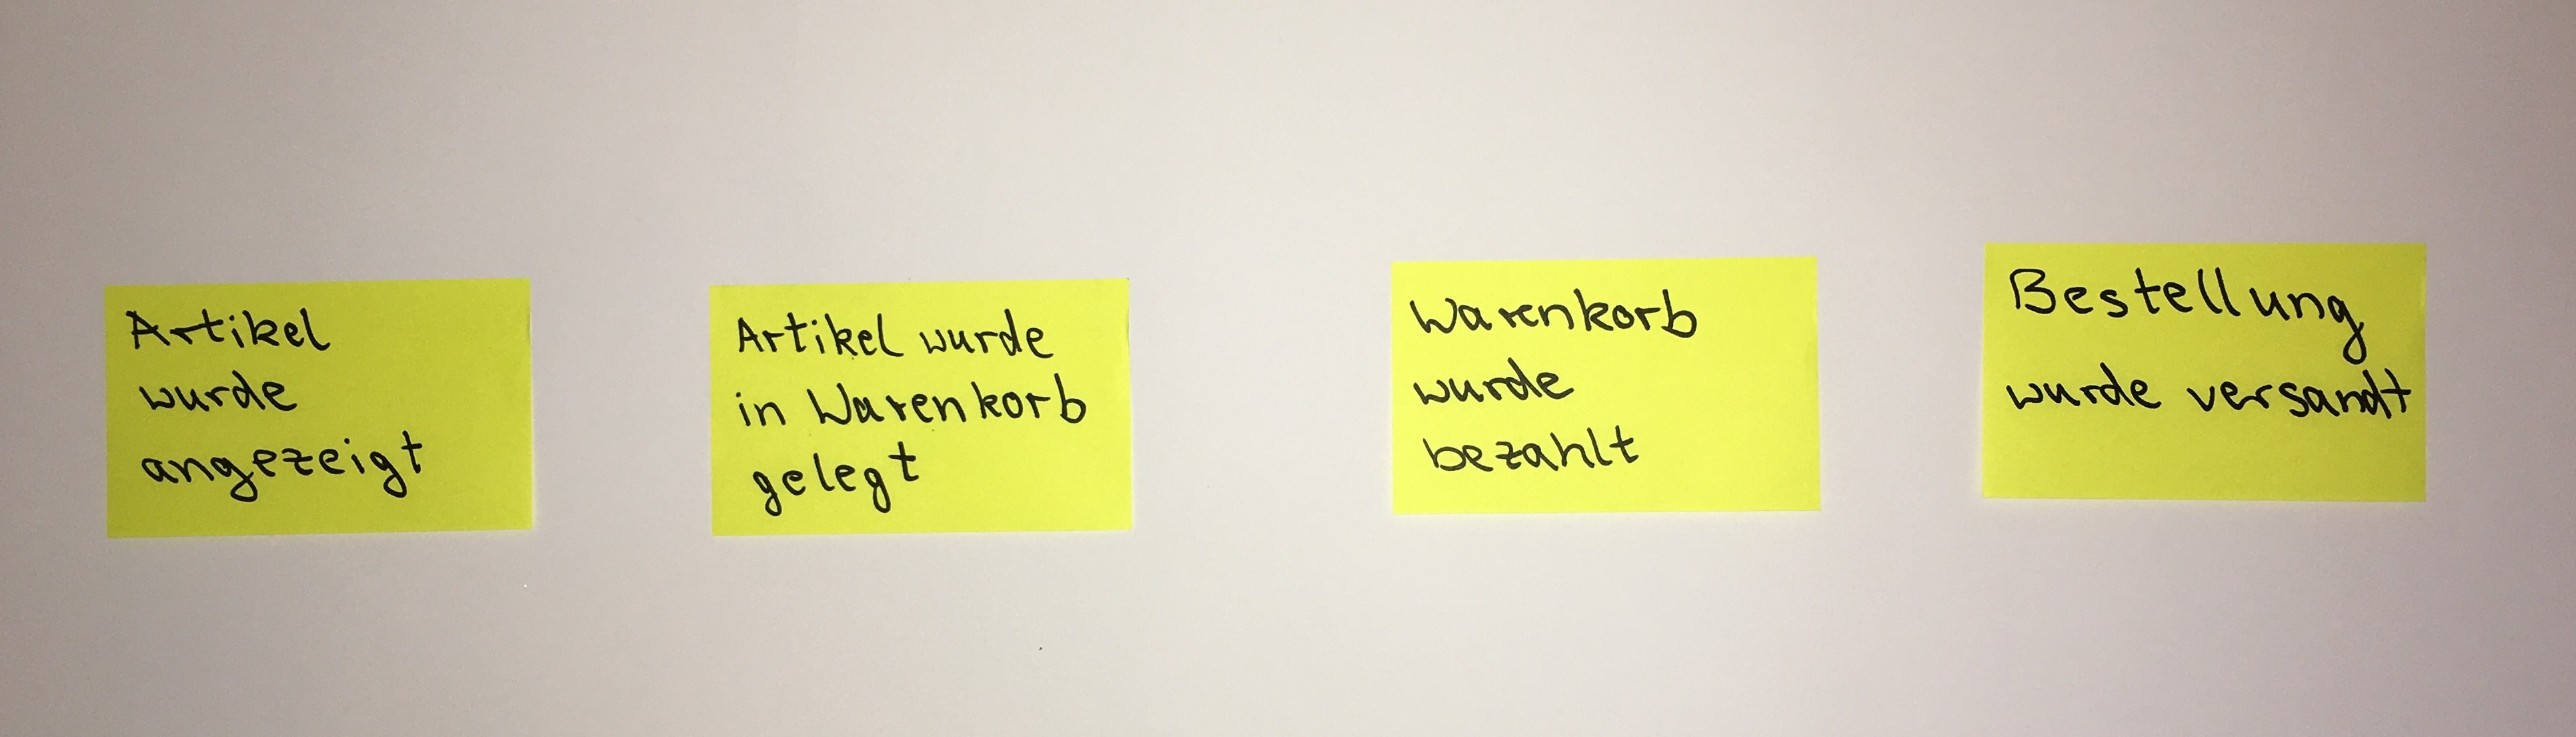
\includegraphics[width=.5\textwidth]{pics/eventstorming_zeitlich_geordnet.jpg}
\end{center}

\end{frame}


%%%%%%%%%%%%%%%%%%%%%%%%%%%%%%%%%%%%%%%%%%%%%%%%%%
%\begin{frame}[fragile]{Übung}

\numberednote{

\textbf{Übung:}

\begin{itemize}

\item Events in zeitliche Reihenfolge bringen

\item Redundanzen entfernen

\item Fehlendes ergänzen

\item Ubiquitous Language erfassen

\item Begriffe schärfen und vereinheitlichen

\end{itemize}

\textbf{Was kann schiefgehen?}

\begin{itemize}
\item x
\end{itemize}

}
%\end{frame}

%%%%%%%%%%%%%%%%%%%%%%%%%%%%%%%%%%%%%%%%%%%%%%%%%%%
%\begin{frame}[fragile]{Was kann schiefgehen?}
%
%\begin{itemize}
%\item x
%\end{itemize}
%
%\end{frame}

%%%%%%%%%%%%%%%%%%%%%%%%%%%%%%%%%%%%%%%%%%%%%%%%%%
\begin{frame}[fragile]{EventStorming III}

\begin{itemize}
\item Vor einem Event muss etwas im System passiert sein:
\item \textbf{Command}
\item Werden in Befehlsform ausgedrückt
\end{itemize}

\end{frame}

%%%%%%%%%%%%%%%%%%%%%%%%%%%%%%%%%%%%%%%%%%%%%%%%%%
\begin{frame}[fragile]{Beispiel}

\begin{center}
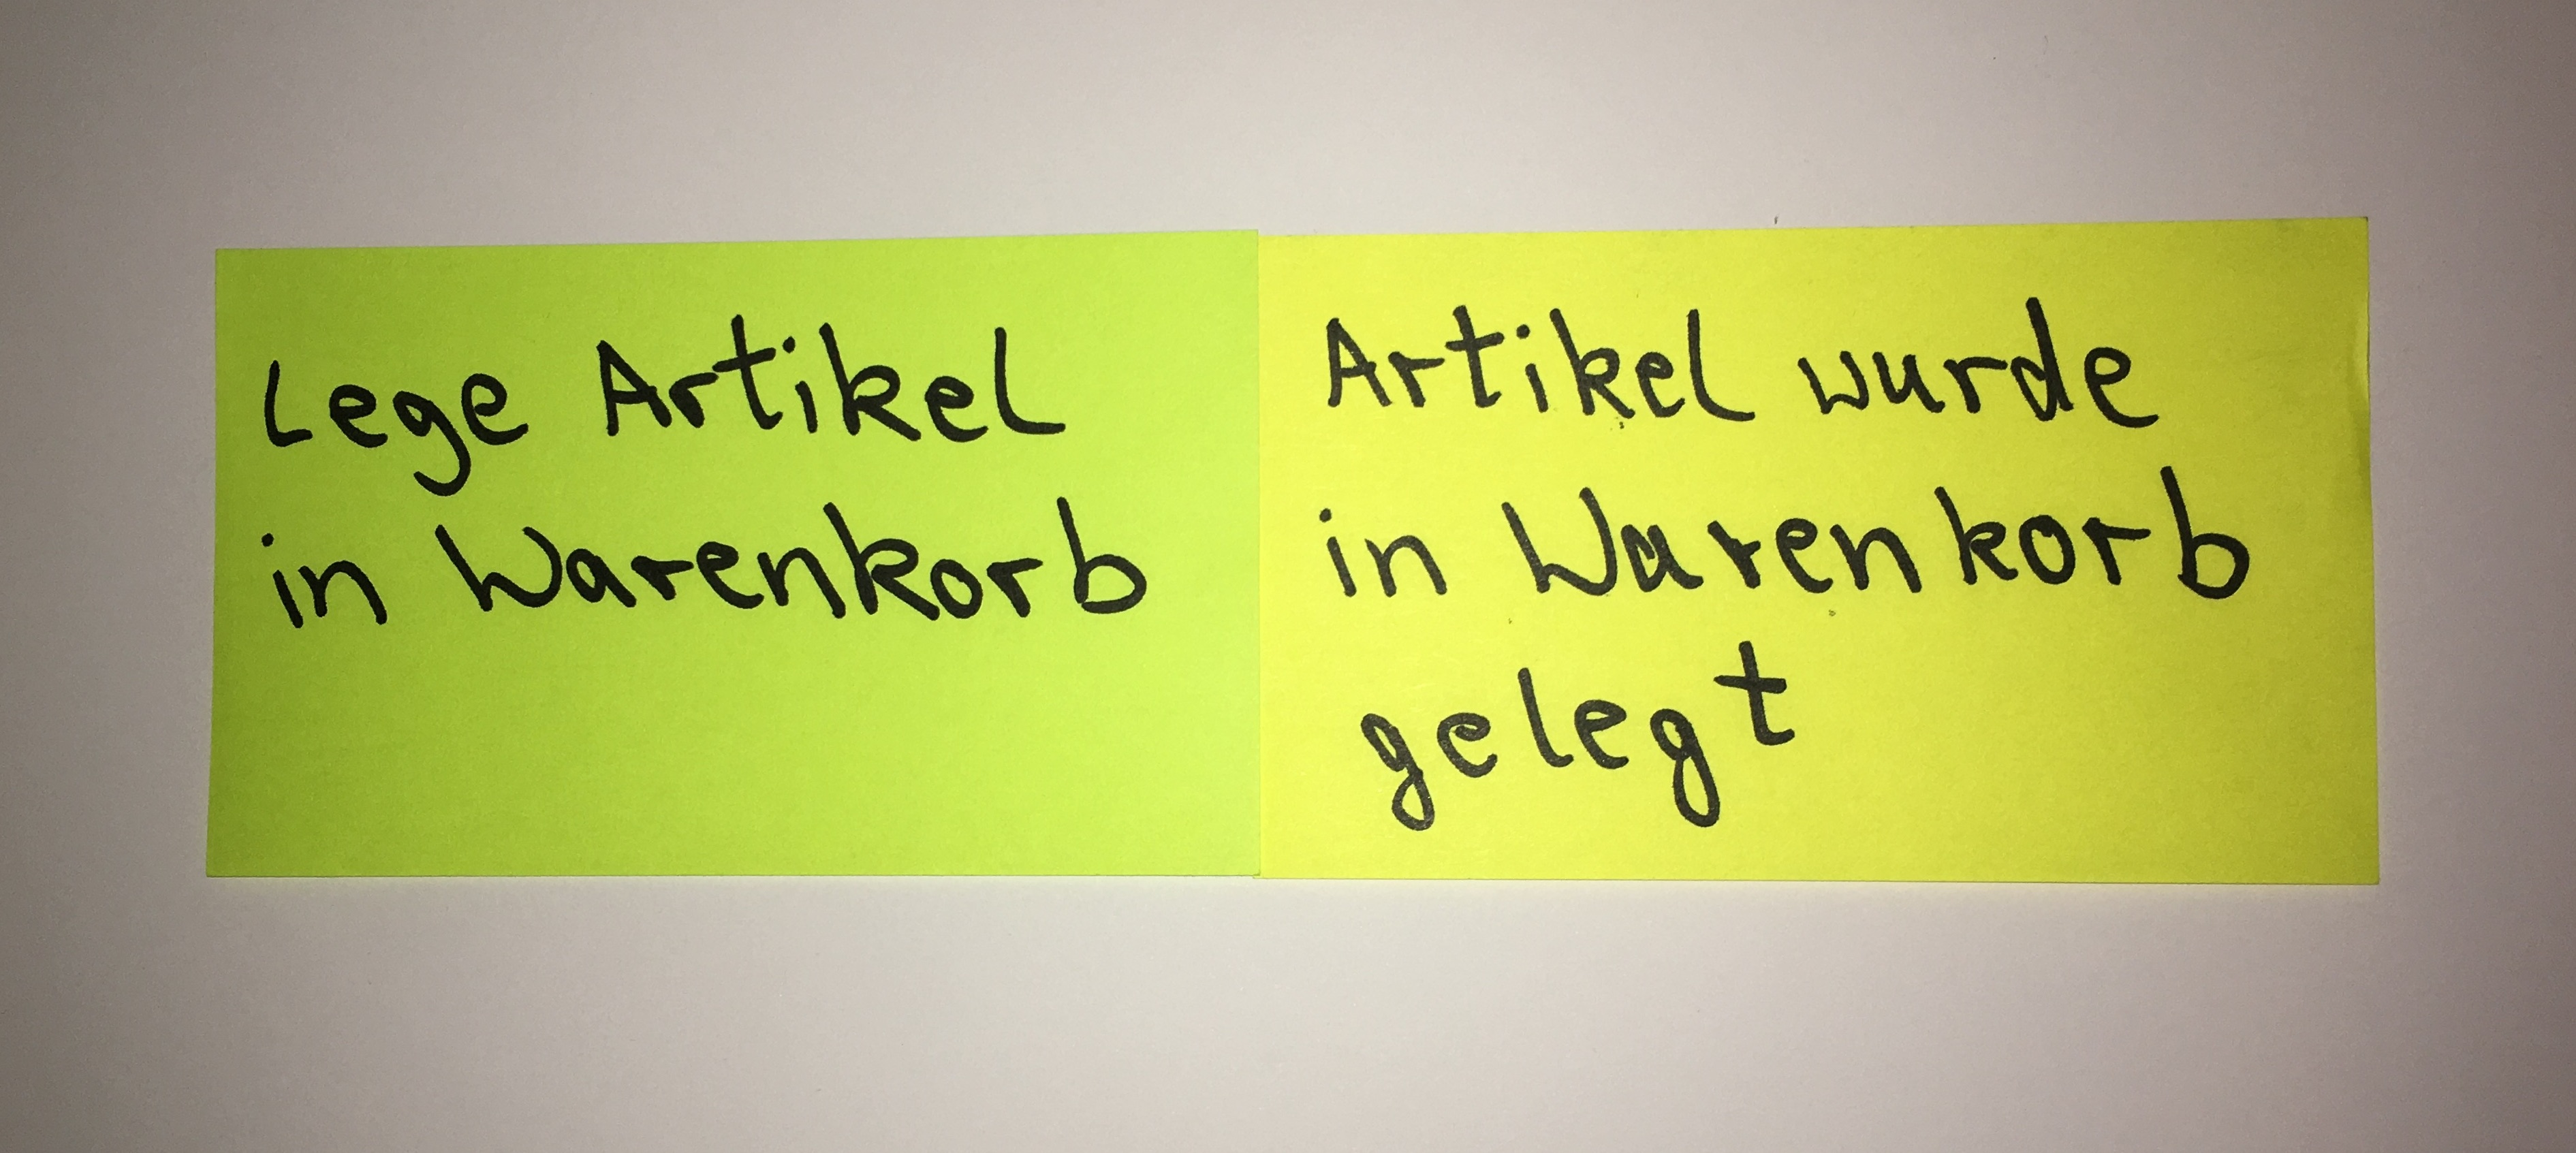
\includegraphics[width=.7\textwidth]{pics/eventstorming2.jpg}
\end{center}

\end{frame}


%%%%%%%%%%%%%%%%%%%%%%%%%%%%%%%%%%%%%%%%%%%%%%%%%%
%%%%%%%%%%%%%%%%%%%%%%%%%%%%%%%%%%%%%%%%%%%%%%%%%%
\begin{frame}[fragile]{EventStorming III}

\begin{itemize}
\item Nicht alle Commands führen direkt zu einem Event
\item \textbf{Constraints} müssen berücksichtigt werden
\end{itemize}

\end{frame}

%%%%%%%%%%%%%%%%%%%%%%%%%%%%%%%%%%%%%%%%%%%%%%%%%%
\begin{frame}[fragile]{Beispiel}

\begin{center}
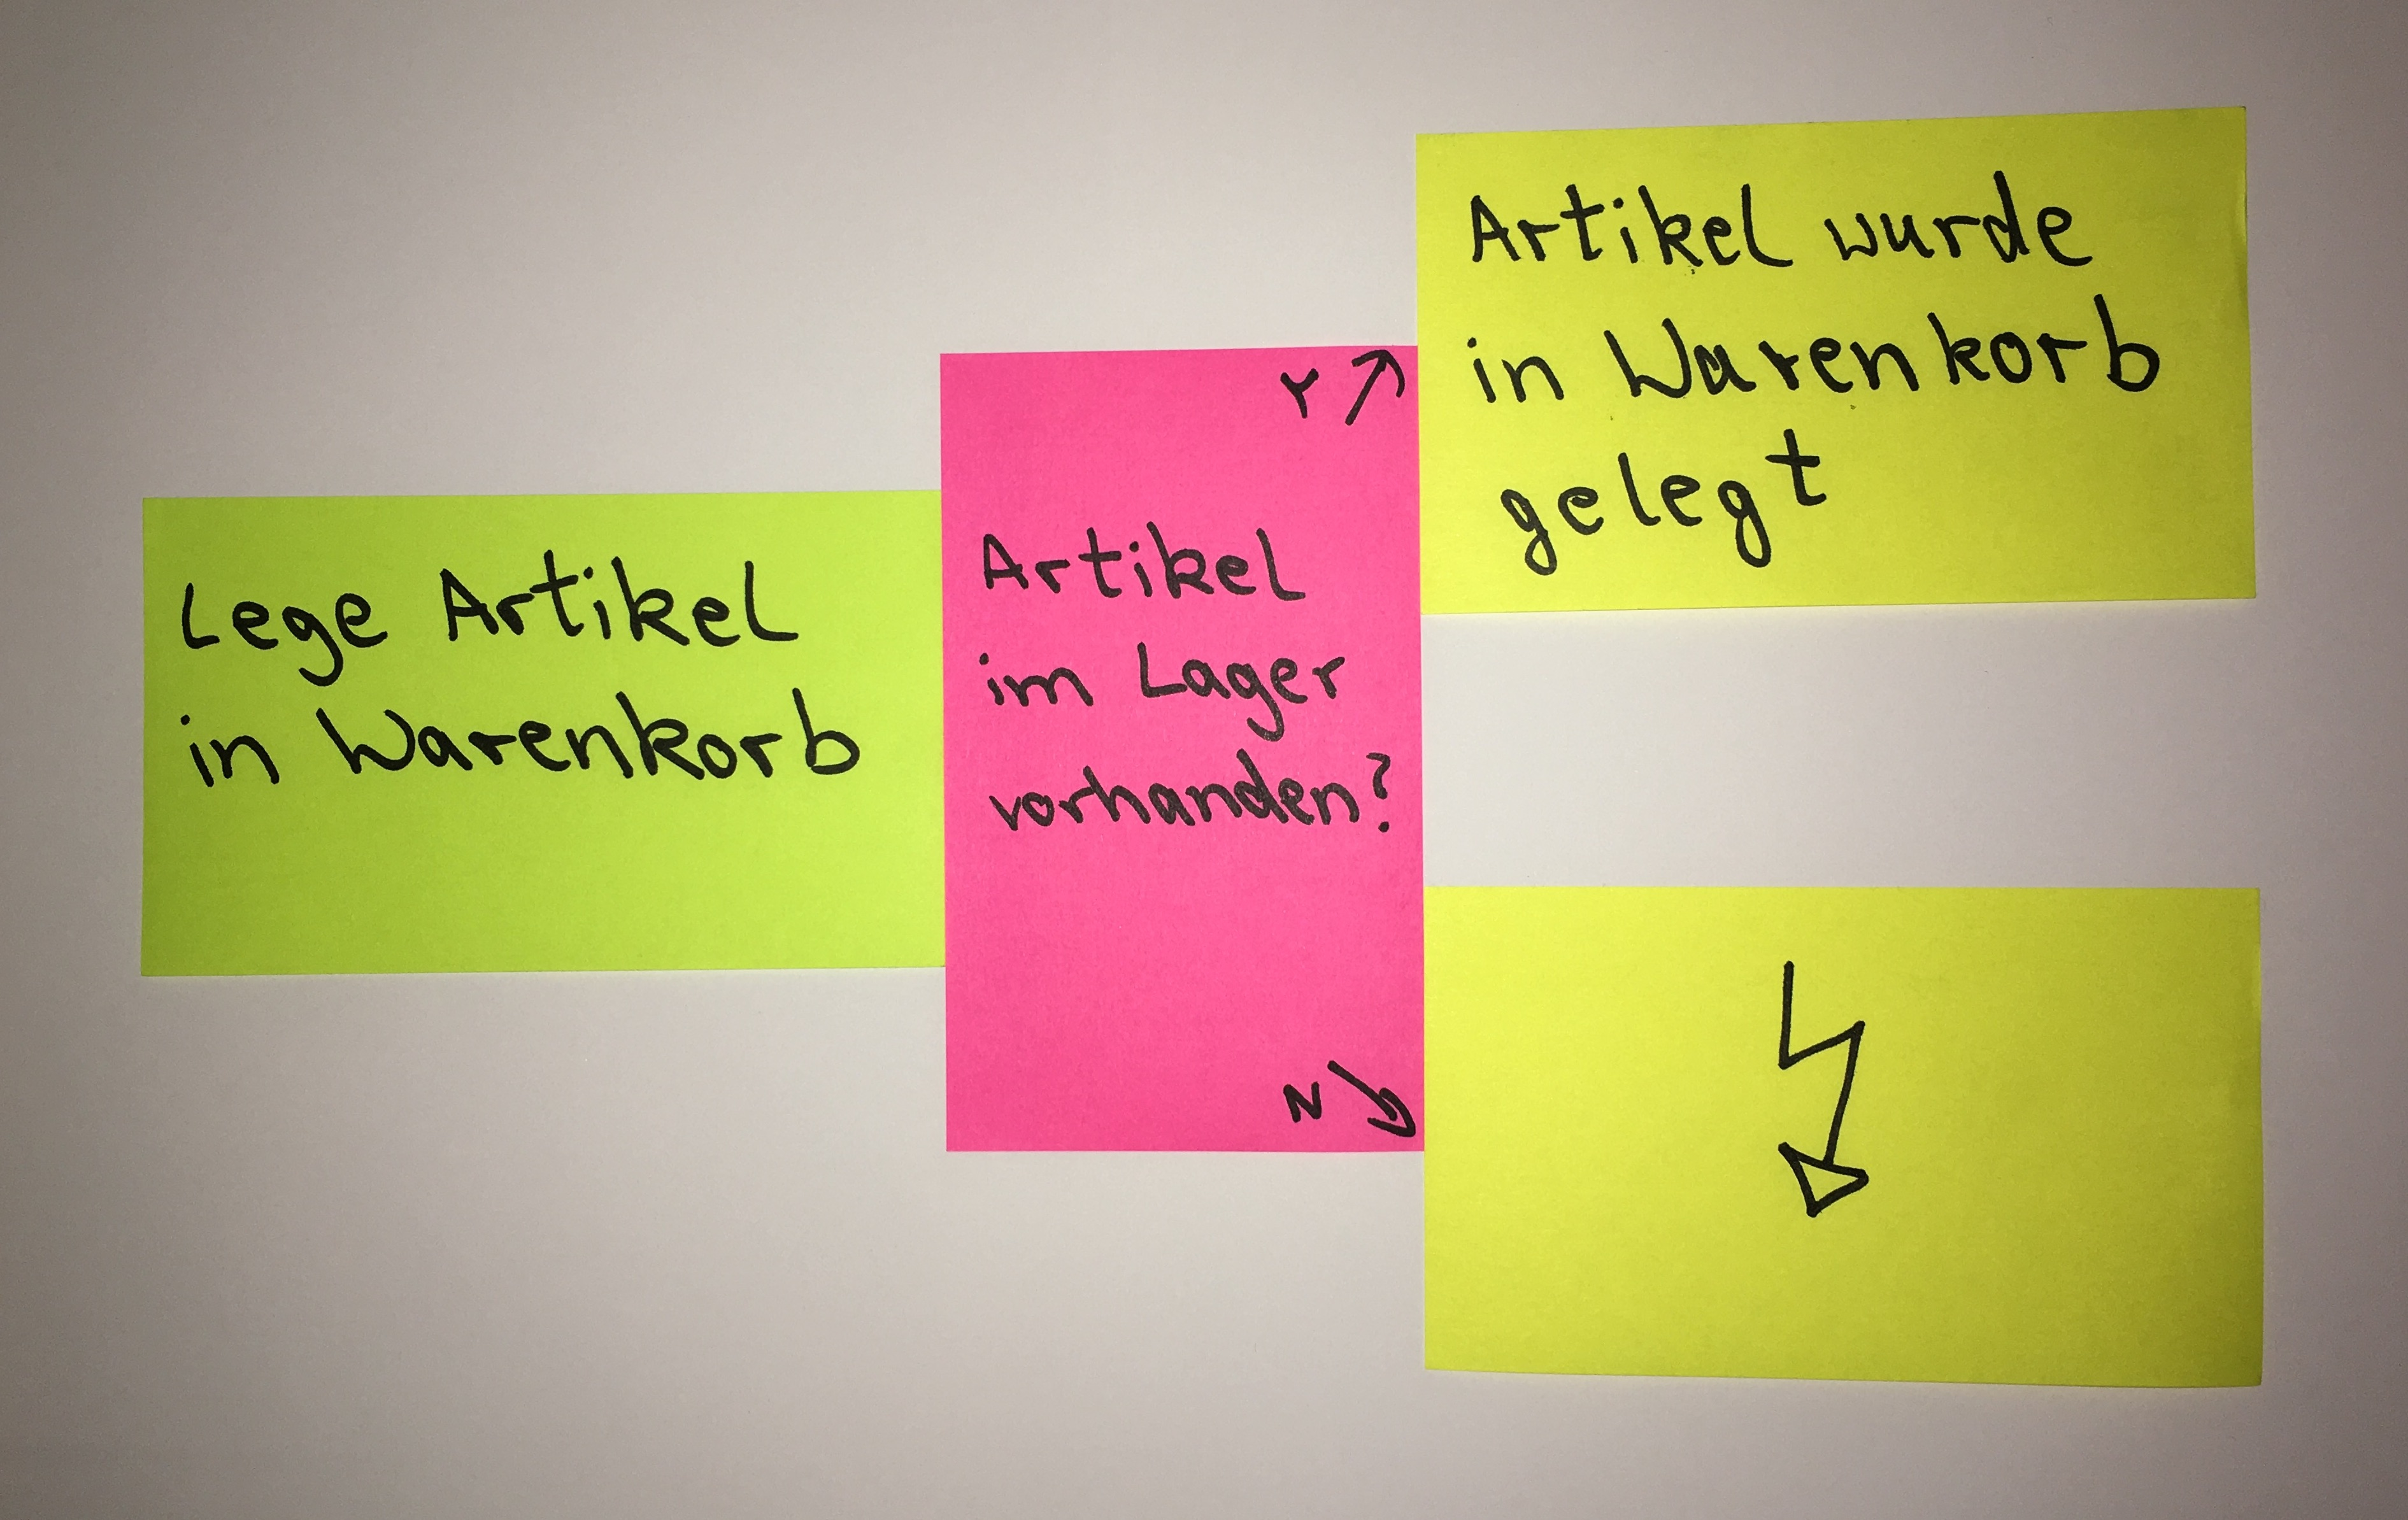
\includegraphics[width=.85\textwidth]{pics/eventstorming3.jpg}
\end{center}

\end{frame}

\numberednote{
\textbf{Übung}

\begin{itemize}
\item Events um Commands und ggf.~auch Constraints ergänzen
\item Fehlendes ergänzen
\end{itemize}

\textbf{Was kann schiefgehen?}

\begin{itemize}
\item x
\end{itemize}

}

%%%%%%%%%%%%%%%%%%%%%%%%%%%%%%%%%%%%%%%%%%%%%%%%%%
%%%%%%%%%%%%%%%%%%%%%%%%%%%%%%%%%%%%%%%%%%%%%%%%%%
\begin{frame}[fragile]{EventStorming IV}

\begin{itemize}
\item Constraints benötigen \textbf{Daten} zur Entscheidung
\item Müssen verfügbar sein
\begin{itemize}
\item Vorherige Erfassung in Event
\item Aus anderem Systemteil
\end{itemize}
\item Fehlen sie, muss das Modell ergänzt werden
\end{itemize}

\end{frame}


%%%%%%%%%%%%%%%%%%%%%%%%%%%%%%%%%%%%%%%%%%%%%%%%%%
\begin{frame}[fragile]{Beispiel}

\begin{center}
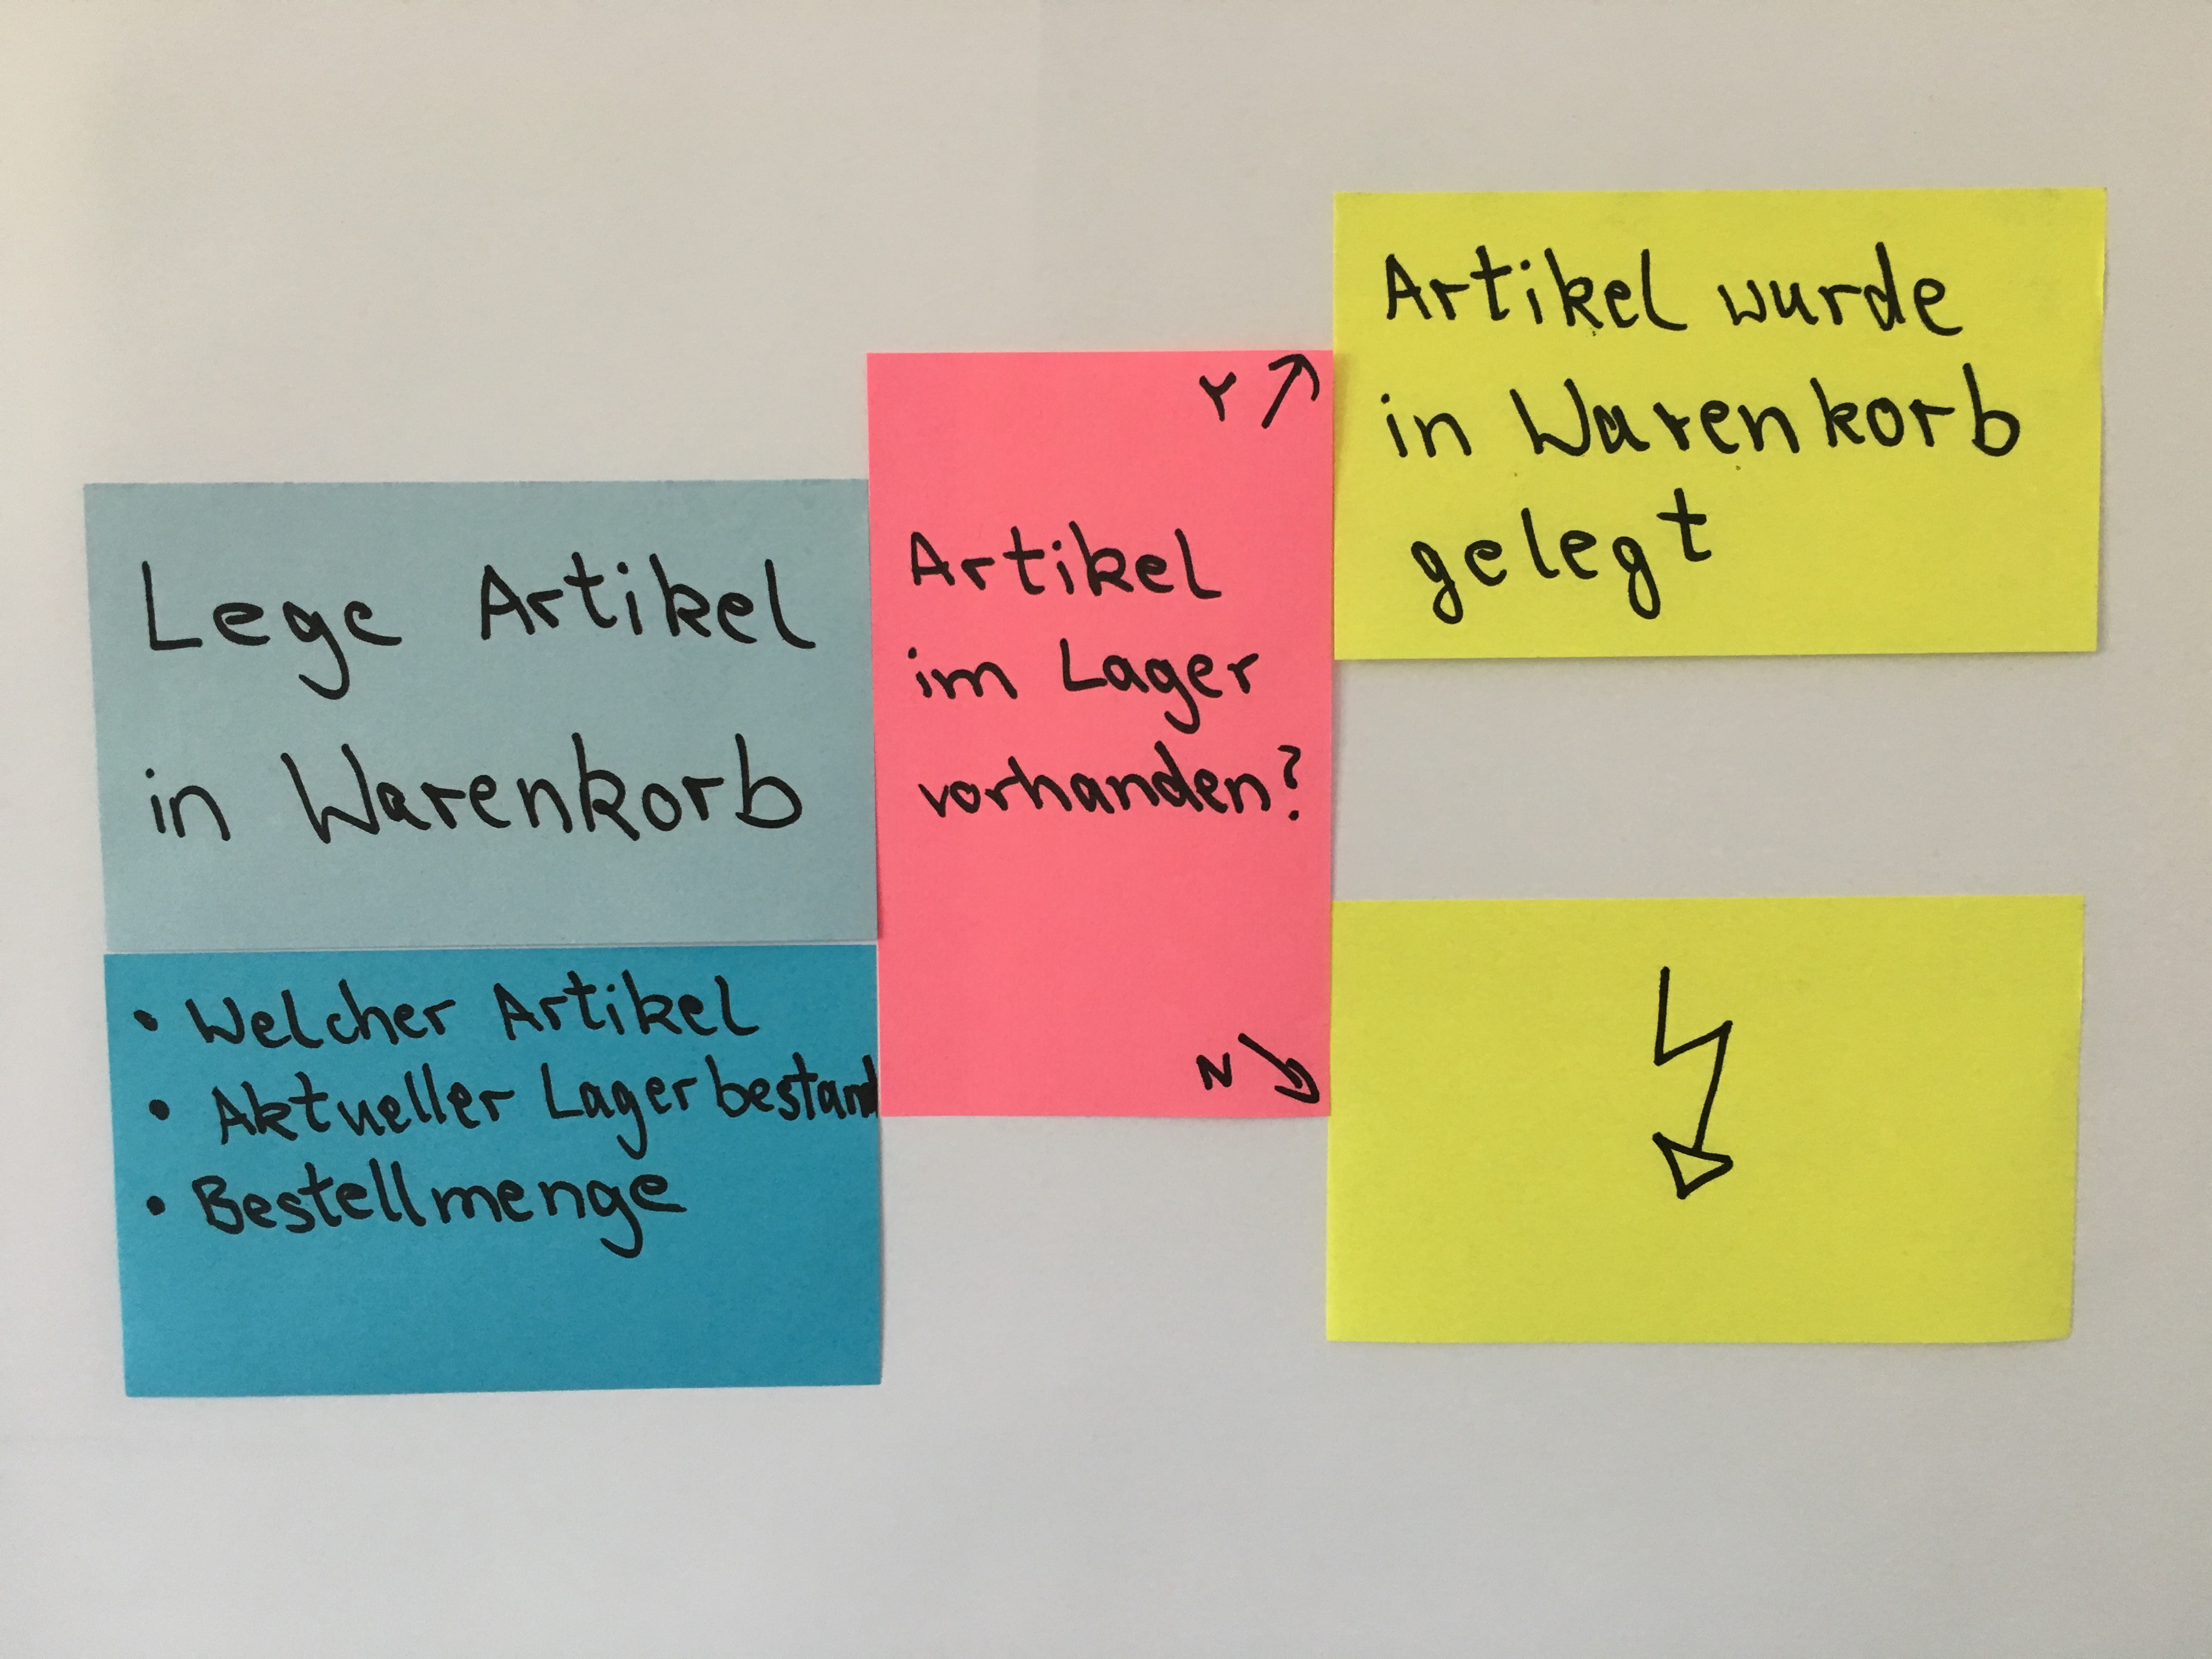
\includegraphics[width=.85\textwidth]{pics/eventstorming4.jpg}
\end{center}

\end{frame}

\numberednote{

\textbf{Übung}

\begin{itemize}
\item In Constraints und Events erforderliche \textbf{Daten} zufügen
\item Fehlendes ergänzen
\end{itemize}

\textbf{Was kann schiefgehen?}

\begin{itemize}
\item x
\end{itemize}

}

%%%%%%%%%%%%%%%%%%%%%%%%%%%%%%%%%%%%%%%%%%%%%%%%%%
%%%%%%%%%%%%%%%%%%%%%%%%%%%%%%%%%%%%%%%%%%%%%%%%%%
\begin{frame}[fragile]{EventStorming V}

\begin{itemize}
\item \textbf{Bounded Contexts}
\begin{itemize}
\item hohe Kopplung \textbf{innerhalb}
\item Wenige Abhängigkeiten \textbf{dazwischen}
\end{itemize}
\item Abhängigkeiten ggf.~mit Wollfäden symbolisieren
\end{itemize}

\end{frame}

\numberednote{
\textbf{Übung}

Identifizieren Sie die Bounded Contexts in Ihrem Modell.

\textbf{Was kann schiefgehen?}

\begin{itemize}
\item x
\end{itemize}

}

%%%%%%%%%%%%%%%%%%%%%%%%%%%%%%%%%%%%%%%%%%%%%%%%%%
%%%%%%%%%%%%%%%%%%%%%%%%%%%%%%%%%%%%%%%%%%%%%%%%%%
\begin{frame}[fragile]{EventStorming VI}

\begin{itemize}
\item \textbf{Entwicklungspakete} (User Stories) ableiten
\item Command mit Events $\Rightarrow$ Story
\begin{itemize}
\item Ggf.~aufteilen in Happy Path + weitere Fälle
\end{itemize}
\end{itemize}

\end{frame}

%%%%%%%%%%%%%%%%%%%%%%%%%%%%%%%%%%%%%%%%%%%%%%%%%%
\begin{frame}[fragile]{Beispiel}

\begin{center}
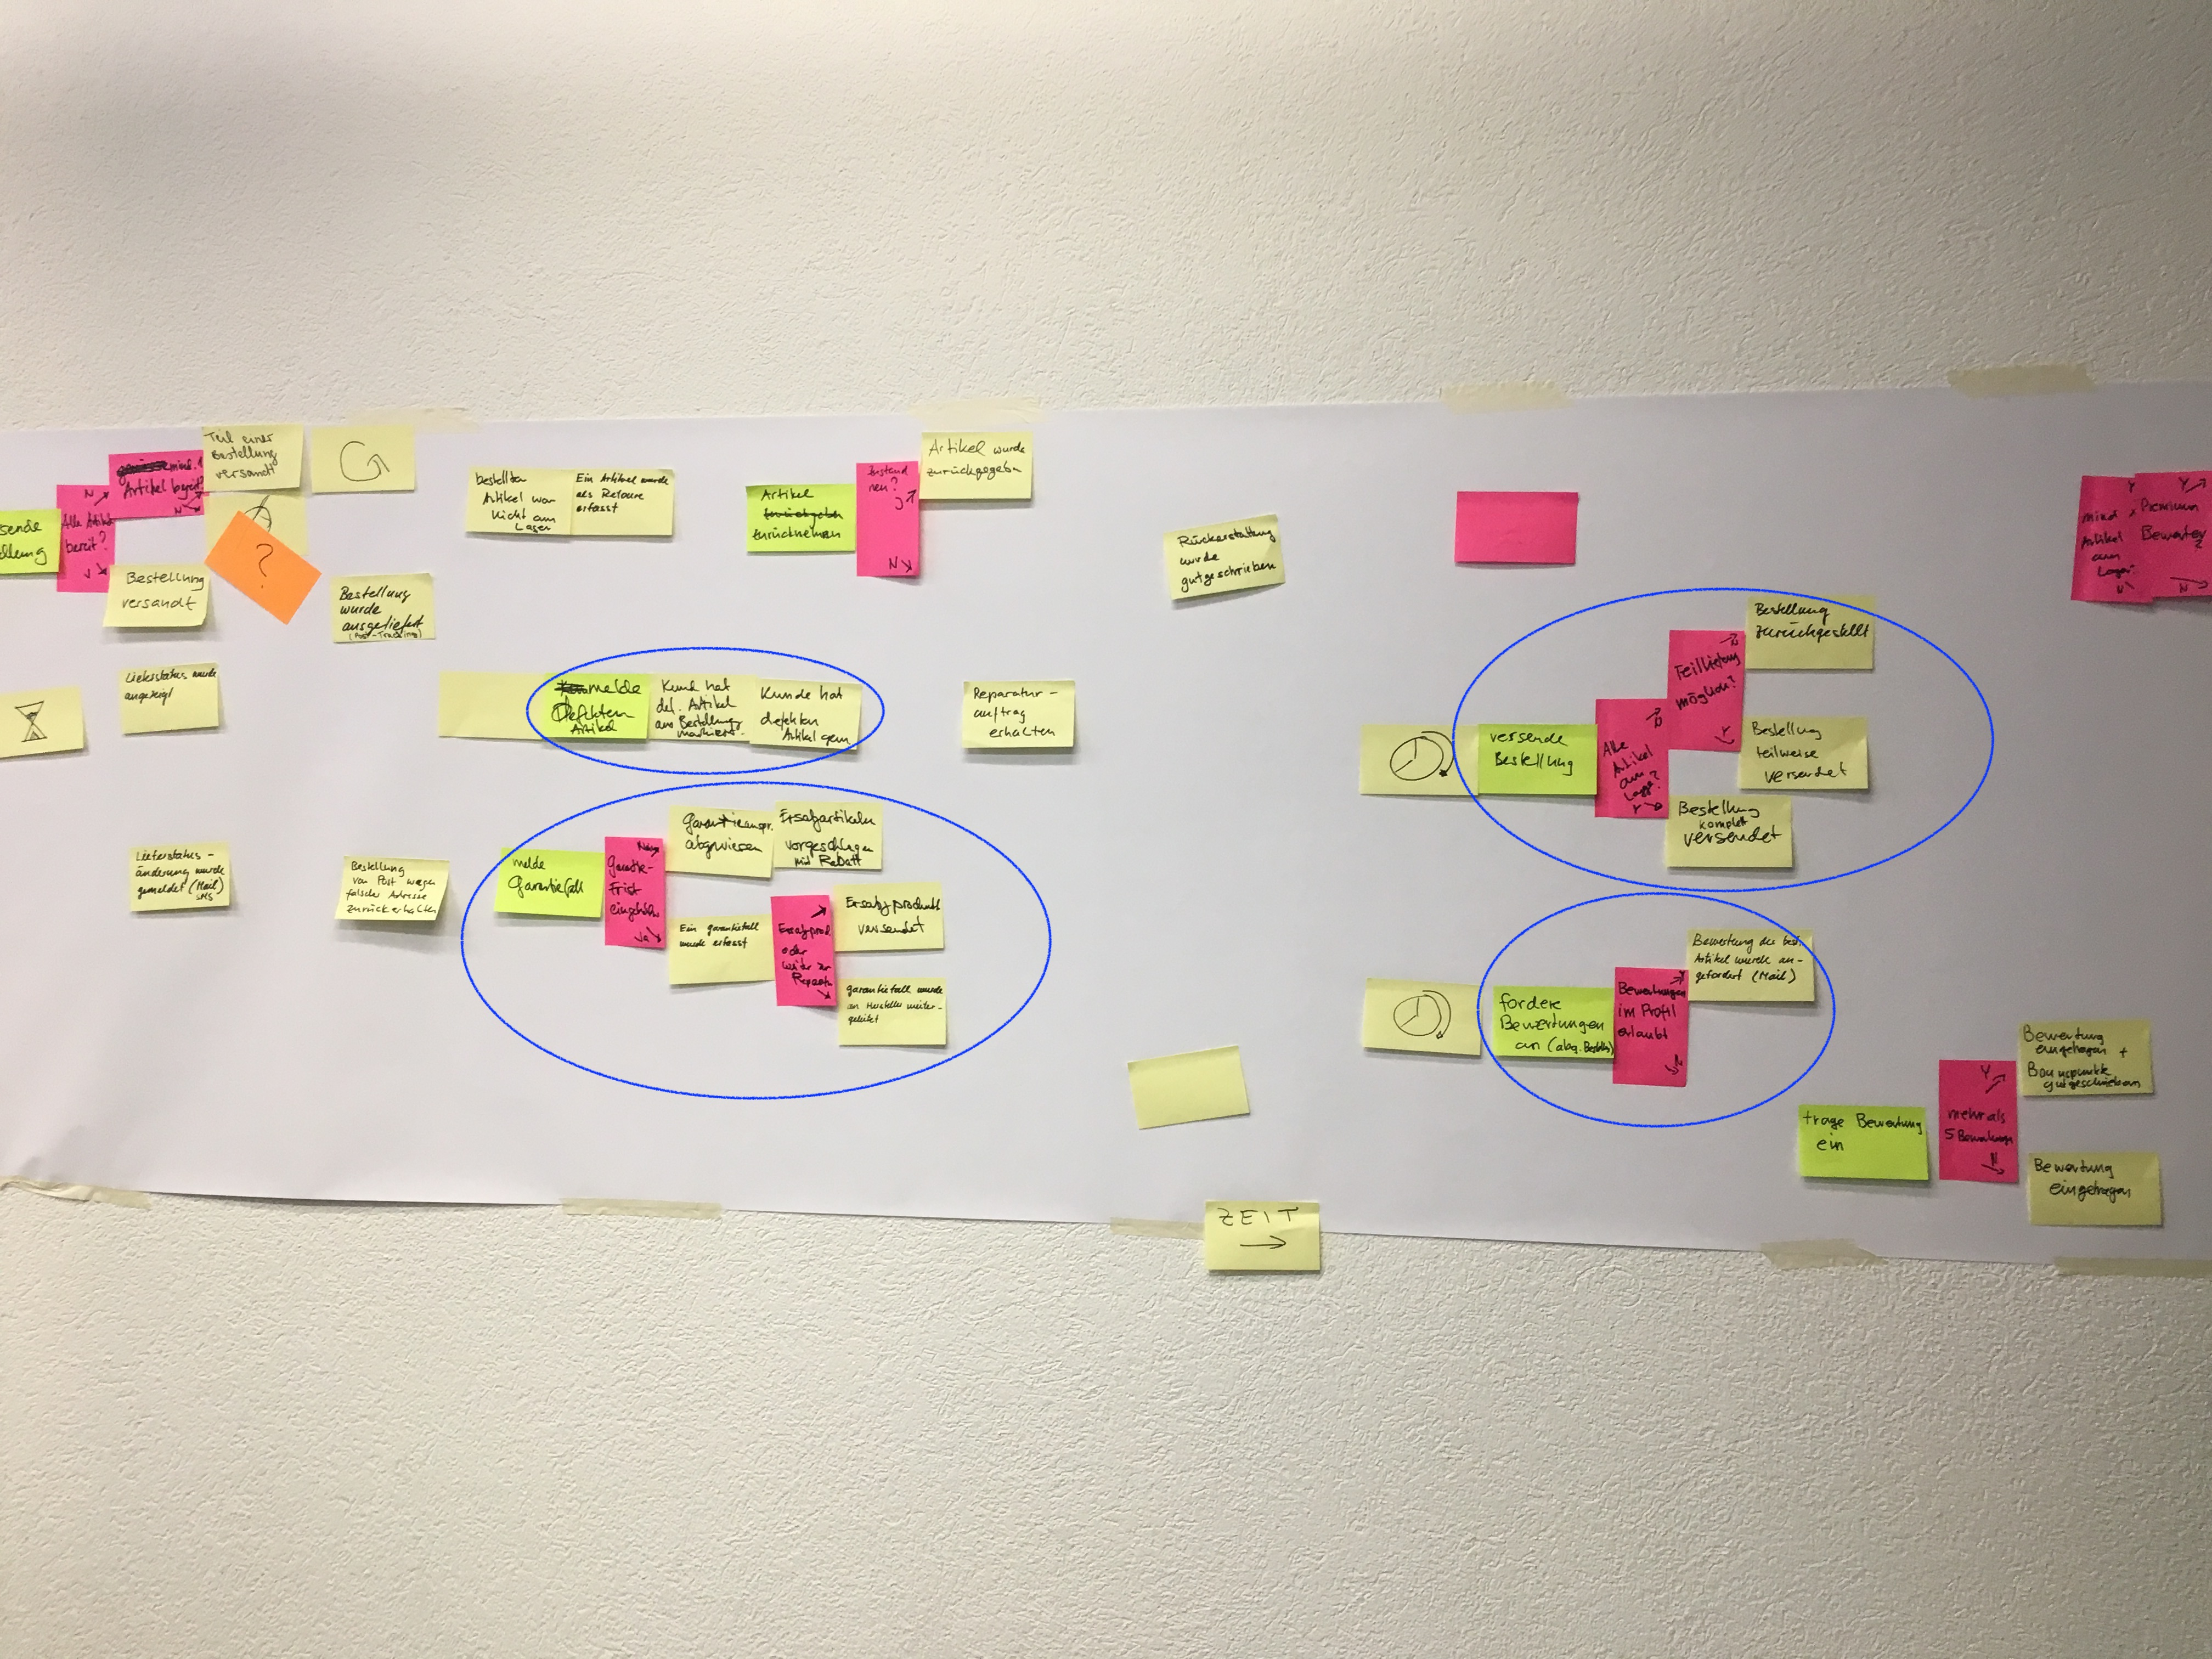
\includegraphics[width=.85\textwidth]{pics/eventstorming_stories.jpg}
\end{center}

\end{frame}

\numberednote{

\textbf{Übung}

Identifizieren Sie User Stories in Ihrem Modell.

\textbf{Was kann schiefgehen?}

\begin{itemize}
\item x
\end{itemize}

}

%%%%%%%%%%%%%%%%%%%%%%%%%%%%%%%%%%%%%%%%%%%%%%%%%%
%%%%%%%%%%%%%%%%%%%%%%%%%%%%%%%%%%%%%%%%%%%%%%%%%%
\begin{frame}[fragile]{Wie geht es weiter?}

Umsetzung einer Story:

\begin{itemize}
\item Zuerst sehr detailliert modellieren
\item Modell an die Wand hängen während der Entwicklung
\item Alle Diskussionen an und mit diesem Modell durchführen
\item Bei Änderungen Modell und Code aktualisieren!
\end{itemize}

\end{frame}







2) Zeitliche Reihenfolge
Redundanzen raus
Fehlendes ergänzen
Ubiquitous Language etablieren

Kritische Fragen:
- Was wenn dies vor jenem passiert?

3) Commands \& Constraints
Commands: Was musste passieren, damit dieses Event stattfinden konnte?
Constraints: Entscheidungen als Frage formulieren, die Events beantworten die Frage
Sauberer modellieren
Clusterbildung
Granularität angleichen
Vollständigkeit checken, Fehlendes ergänzen

Kritische Fragen:
- Folgt dies immer direkt? Gibt es hier keine Constraints?

- Wenn keine Constraints: Entweder Domäne langweilig oder Problem noch nicht verstanden

- Darstellung von Zeit
- Darstellung von Wiederholung

4) Daten zufügen, die bei Entscheidungen und für die Events benötigt werden
Fehlendes ergänzen
Datenquellen identifizieren
Verbindungen schaffen


Debrief

%%%%%%%%%%%%%%%%%%%%%%%%%%%%%%%%%%%%%%%%%%%%%%%%%%
\begin{frame}[fragile]{Warum Modellieren?}

\begin{itemize}
\item Modellieren dient dazu, Gedanken sichtbar und \glqq begreifbar\grqq{} zu machen
\onslide+<2->
\item Jeder entwickelt eigene Vorstellungen von etwas Gehörtem
\item Das gilt übrigens auch für diesen Kurs!
\onslide+<3->
\item Ein Modell versucht Klarheit zu schaffen
\item EventStorming ist ein Weg, sehr schnell zu einem sehr detaillierten Modell zu kommen
\end{itemize}

\end{frame}

%%%%%%%%%%%%%%%%%%%%%%%%%%%%%%%%%%%%%%%%%%%%%%%%%%
\begin{frame}[fragile]{Grundsätzliches}

\begin{itemize}
\item Alles mit dem Fachbereich abklären
\item Immer wieder kritisch hinterfragen!
\item Immer wieder Alternativen diskutieren!
\item \glqq Was wenn dies vor jenem passiert?\grqq
\item Die üblichen Verdächtigen (\glqq immer\grqq, \glqq nie\grqq, \glqq kann nicht sein\grqq{} \ldots) entkräften
\end{itemize}

\end{frame}

%%%%%%%%%%%%%%%%%%%%%%%%%%%%%%%%%%%%%%%%%%%%%%%%%%
\begin{frame}[fragile]{Einsichten in die Domäne gewinnen}
\begin{itemize}
\item Kollaboration zwischen Fachbereich und Entwicklern ist der entscheidende Faktor für den Erfolg eines Projekts
\item Man braucht die Domänen-Experten des betreffenden Bereiches
\end{itemize}

\end{frame}


EventStorming auch außerhalb von DDD einsetzbar



Wie geht's weiter?
- Stories schneiden -> Einzel-EventStorming
- Implementieren
- Event Sourced implementieren


%%%%%%%%%%%%%%%%%%%%%%%%%%%%%%%%%%%%%%%%%%%%%%%%%%
\begin{frame}[fragile]{}

\begin{itemize}
\item x
\end{itemize}

\end{frame}

%%%%%%%%%%%%%%%%%%%%%%%%%%%%%%%%%%%%%%%%%%%%%%%%%%
\begin{frame}[fragile]{}

\begin{center}
{
\LARGE
}
\end{center}

\end{frame}

%%%%%%%%%%%%%%%%%%%%%%%%%%%%%%%%%%%%%%%%%%%%%%%%%%
\begin{frame}[fragile]{}

\begin{center}
%\includegraphics[width=\textwidth]{pics/.jpg}
\end{center}

\end{frame}


%%%%%%%%%%%%%%%%%%%%%%%%%%%%%%%%%%%%%%%%%%%%%%%%%%
\begin{frame}{Vielen Dank!}

        Folien: \url{https://github.com/NicoleRauch/} 
        
        ~\\[1em]
        \begin{block}{Nicole Rauch}
        \begin{description}[Twitterxx]
                \item[E-Mail]  \href{mailto:info@nicole-rauch.de}{\texttt{info@nicole-rauch.de}}
                \item[Twitter] \href{http://twitter.com/NicoleRauch}{\texttt{@NicoleRauch}}
                \item[Web] \href{http://www.nicole-rauch.de}{\texttt{http://www.nicole-rauch.de}}
        \end{description}
        \end{block}
        
        EventStorming und DDD $\cdot$ Training $\cdot$ Coaching $\cdot$ Facilitation
\end{frame}

%%%%%%%%%%%%%%%%%%%%%%%%%%%%%%%%%%%%%%%%%%%%%%%%%%
\begin{frame}{Credits}

Palm Beach: Grand Velas Riviera Maya - Beach Palm Trees Riviera Maya \\
{\footnotesize \url{https://www.flickr.com/photos/grandvelasrivieramaya/3179390917}}

Crowded Beach: Deyvis Tejada - Cala Mondrago - Cala Esmeralda Mallorca  \\
{\footnotesize \url{https://www.flickr.com/photos/143430050@N02/33639336432}}

Japan Beach: Aleksander Dragnes - Miyajima Floating Torii  \\
{\footnotesize \url{https://www.flickr.com/photos/adragnes/644727155}}

Ice Beach: Kitty Terwolbeck - Colorful waters (Spitsbergen 2012)  \\
{\footnotesize \url{https://www.flickr.com/photos/kittysfotos/7902630982}}

Onlineshopping: Elaine Smith - Online Shopping \\
{\footnotesize \url{https://www.flickr.com/photos/155416046@N05/35933760125}}

Warehouse: Gwan Kho - Mediq Sverige Kungsbacka warehouse \\
{\footnotesize \url{https://www.flickr.com/photos/gwankho/6205837092}}

Ordering: cybrgrl - Invoices \\
{\footnotesize \url{https://www.flickr.com/photos/cybrgrl/2693815369}}


{\footnotesize \url{}}
{\footnotesize \url{}}
{\footnotesize \url{}}

\end{frame}


